\documentclass[a4paper,12pt]{report}
\usepackage[english]{babel}
\usepackage[utf8]{inputenc}
\usepackage[T1]{fontenc}
\usepackage[top=2cm, bottom=2cm, left=2cm, right=2cm]{geometry}
\usepackage{graphicx}
\usepackage{hyperref}
\usepackage{float}
\usepackage{amsmath,amssymb}
\usepackage{array,tabularx,booktabs,multirow}
\usepackage{setspace}
\usepackage{caption,subcaption}
\usepackage{enumitem}
\usepackage{xcolor}
\usepackage{url}
\usepackage{tikz}
\usetikzlibrary{arrows.meta, positioning, shapes.geometric, shapes.multipart, calc, backgrounds, fit}

\raggedbottom

\setcounter{secnumdepth}{3}
\setcounter{tocdepth}{3}

\hypersetup{
  pdfauthor={ENSIAS - 2IA},
  pdftitle={MLOps Pipeline for Edge Melanoma Detection},
  pdfsubject={End-of-Year Project Report},
  pdfkeywords={MLOps, Melanoma, ONNX, Docker, CI/CD},
  pdfstartview={FitH}
}

\begin{document}
\newcommand{\HRule}{\rule{\linewidth}{0.5mm}}

\begin{titlepage}
\begin{center}


\includegraphics[width=0.6\textwidth]{./ensiass.png}~\\[1.5cm]

\textsc{\Large MOHAMMED V UNIVERSITY IN RABAT}\\[0.3cm]
\textsc{\Large National School of Computer Science and Systems Analysis}\\[0.3cm]
\textsc{\Large ENSIAS}\\[2cm]

\textsc{\huge \bfseries End-of-Year Project Report}\\[0.5cm]
\textsc{\Large Artificial Intelligence Engineering -- 2IA}\\[1.5cm]

\HRule \\[0.4cm]
{\huge \bfseries MLOps Pipeline for}\\[0.2cm]
{\huge \bfseries Edge-Deployable Melanoma Detection}\\[0.4cm]
\HRule \\[2cm]

\begin{minipage}[t]{0.45\textwidth}
\begin{flushleft} \large
\emph{Prepared by:}\\[0.5cm]
[Student Name]\\
\end{flushleft}
\end{minipage}
\hfill
\begin{minipage}[t]{0.45\textwidth}
\begin{flushright} \large
\emph{Supervised by:}\\[0.5cm]
[Professor Name]\\
\end{flushright}
\end{minipage}

\vfill
{\large Academic Year 2025/2026}
\end{center}
\end{titlepage}

\newpage ~ \thispagestyle{empty} \newpage

\pagenumbering{roman}
\begin{center}
\vspace*{3cm}
\textsc{\huge \bfseries Acknowledgments}\\[1cm]
\end{center}

\begin{spacing}{1.3}

We would like to express our sincere gratitude to everyone who supported and guided us throughout this end-of-year project. First and foremost, we extend our thanks to the National School of Computer Science and Systems Analysis (ENSIAS) and the Artificial Intelligence Engineering (2IA) programme for providing the academic environment and resources necessary to undertake a project of this scope.

We are especially grateful to our project supervisor for their invaluable mentorship, technical guidance, and encouragement throughout every phase of this work. Their expertise in MLOps best practices and machine learning engineering shaped the quality and direction of this project. We also thank all the teaching staff at ENSIAS whose courses on deep learning, software engineering, and DevOps laid the foundation upon which this project is built.

\end{spacing}

\newpage
\begin{center}
\vspace*{3cm}
\textsc{\huge \bfseries Abstract}\\[1cm]
\end{center}

\begin{spacing}{1.3}

This report presents a comprehensive, end-to-end MLOps pipeline for melanoma detection on edge devices. The pipeline spans the full machine learning lifecycle -- from data ingestion through CI/CD -- applying modern software engineering practices to produce a reproducible, production-ready system.

The pipeline uses the HAM10000 dataset (10,015 dermoscopic images, 7 classes) with patient-aware GroupShuffleSplit on lesion identifier to prevent data leakage. Data quality is enforced through Great Expectations with 7 validation expectations and 100\% image integrity verification. Three convolutional architectures were trained and compared: EfficientNet-B0 achieved the highest ROC-AUC of 0.91 (4.3M parameters), followed by ResNet50 at 0.84 (24M) and MobileNetV3-Small at 0.84 (1.5M). At the clinically-calibrated threshold of 0.15, sensitivity reaches 80.6\% with specificity of 82.8\%. The best-performing model was exported to ONNX (FP32, 16.6~MB) achieving a mean inference latency of 6.7~ms and p99 latency of 10.3~ms on CPU. Post-training INT8 quantisation was investigated across five strategies but proved incompatible with EfficientNet-B0, producing 10--15\% AUC degradation due to SiLU activation and depthwise separable convolution incompatibility with integer arithmetic.

The deployment architecture centres on a FastAPI inference server with 6 endpoints, containerised through Docker multi-stage builds. CI/CD is orchestrated via GitHub Actions with 41 passing tests across 5 pipeline stages. An interactive Gradio demonstration is hosted on Hugging Face Spaces. Explainability is provided through Grad-CAM visualisation, MC-Dropout uncertainty quantification, and temperature scaling calibration. This project demonstrates that MLOps provides the engineering framework to transform a research model into a robust, edge-deployable clinical decision support tool.

\end{spacing}

\newpage
\begin{center}
\vspace*{3cm}
\textsc{\huge \bfseries List of Abbreviations}\\[1cm]
\end{center}

\begin{spacing}{1.3}
\begin{table}[H]
\centering
\begin{tabular}{ll}
\toprule
\textbf{Abbreviation} & \textbf{Meaning} \\
\midrule
MLOps    & Machine Learning Operations \\
CI/CD    & Continuous Integration / Continuous Deployment \\
DVC      & Data Version Control \\
GE       & Great Expectations \\
ONNX     & Open Neural Network Exchange \\
INT8     & 8-bit Integer (Quantisation) \\
FP32     & 32-bit Floating Point \\
AUC      & Area Under the ROC Curve \\
ECE      & Expected Calibration Error \\
CNN      & Convolutional Neural Network \\
LR       & Learning Rate \\
AdamW    & Adaptive Moment Estimation with Weight Decay \\
Grad-CAM & Gradient-weighted Class Activation Mapping \\
MC       & Monte Carlo \\
HAM10000 & Human Against Machine with 10000 training images \\
ISIC     & International Skin Imaging Collaboration \\
REST     & Representational State Transfer \\
API      & Application Programming Interface \\
TTL      & Time-To-Live \\
LRU      & Least Recently Used \\
SHA-256  & Secure Hash Algorithm (256-bit) \\
QDQ      & Quantise-Dequantise (ONNX operators) \\
\bottomrule
\end{tabular}
\end{table}
\end{spacing}

\newpage

\listoffigures
\newpage
\tableofcontents
\newpage

\pagenumbering{arabic}
\setcounter{page}{1}

\chapter{General Introduction}
\begin{spacing}{1.3}

Machine learning has undergone a profound transformation over the past decade. What began as a domain of academic research, confined to notebooks and controlled laboratory environments, has matured into a critical component of enterprise software systems. The narrative has shifted: organisations no longer ask whether they can build a model, but whether they can deploy, monitor, and maintain it at scale. This evolution mirrors the broader trajectory of software engineering, where the introduction of DevOps practices revolutionised the reliability and velocity of software delivery.

Despite significant advances in model architectures, frameworks, and hardware accelerators, the bridge between a trained model and a production system remains fragile. A frequently cited statistic in the MLOps community is that 87\% of machine learning models never reach production. The reasons are manifold: brittle data pipelines, unreproducible training procedures, absence of monitoring, model decay over time, and a cultural divide between data scientists and software engineers. Sculley et al.~\cite{sculley2015} described this phenomenon as \textit{hidden technical debt} in machine learning systems, arguing that the ML component itself is a tiny fraction of the overall system, surrounded by vast infrastructure for data collection, feature extraction, configuration, monitoring, and serving.

MLOps -- a portmanteau of Machine Learning and Operations -- extends the principles of DevOps to the unique challenges of ML systems. At its core, MLOps advocates for automated testing and validation of data, code, and models on every change (Continuous Integration), automated deployment pipelines moving models from training to serving (Continuous Delivery), automated retraining triggered by data drift (Continuous Training), versioning of data, models, experiments, and configurations, and production observability of model performance and system health. The MLOps maturity model proposed by Google~\cite{google_mlops} defines three levels, from manual script-driven processes to full CI/CD automation.

Healthcare applications occupy a uniquely demanding position in the machine learning landscape. Unlike recommendation systems where failure results in lost revenue, failures in medical AI can result in misdiagnosis and patient harm. The stakes demand safety mechanisms that degrade gracefully under uncertainty, full reproducibility where every prediction is traceable to its training pipeline, and continuous monitoring to detect silent model degradation. MLOps provides the operational framework to satisfy these requirements, making it not a luxury but a prerequisite in medical AI.

Melanoma is the deadliest form of skin cancer, accounting for approximately 75\% of skin cancer-related deaths despite representing only 1\% of diagnoses. The prognosis is starkly bifurcated by stage at detection: early-stage detection yields a 5-year survival rate exceeding 99\%, while late-stage detection drops survival below 30\%. Dermoscopy improves diagnostic accuracy over naked-eye examination but requires significant training. Dermatologists are in short supply globally, with particularly acute shortages in rural and underserved communities. Automated screening systems deployed on edge devices -- smartphones, tablets, or Raspberry Pi devices -- offer a compelling solution by enabling offline, low-cost, real-time screening without cloud dependency, preserving data privacy in the process.

This project is a research and educational prototype, not a medical device. It has not been evaluated by any regulatory authority. The pipeline is designed with safety guardrails -- uncertainty quantification, confidence thresholds, and mandatory clinical review flags -- that align with regulatory best practices. The HAM10000 dataset~\cite{tschandl2018}, comprising 10,015 dermoscopic images across seven diagnostic categories, serves as the training and evaluation foundation.

The present report documents the design, implementation, and evaluation of a complete 12-phase MLOps pipeline for melanoma detection, spanning data ingestion through edge deployment. Chapter~2 presents the clinical context, dataset characteristics, pipeline architecture, and model architectures. Chapter~3 reviews the state of the art in MLOps platforms, melanoma detection literature, and edge inference optimisation. Chapter~4 defines functional, non-functional, and MLOps-specific requirements. Chapter~5 provides a detailed, phase-by-phase account of the entire implementation. Chapter~6 presents model performance results and the Gradio frontend interface. Chapter~7 assesses project achievements against requirements, and the conclusion outlines directions for future work.

\end{spacing}


\chapter{Project Context}
\begin{spacing}{1.3}

\section{Clinical Background}

Melanoma ranks as the most lethal form of skin cancer, responsible for the overwhelming majority of skin cancer fatalities worldwide. According to the American Cancer Society, approximately 100,000 new cases of invasive melanoma are diagnosed annually in the United States alone, with over 8,000 deaths attributed to the disease each year. Global incidence has risen steadily over the past three decades, with particularly sharp increases in fair-skinned populations exposed to high levels of ultraviolet radiation.

The prognosis for melanoma patients is dramatically stage-dependent. Early-stage detection (Stage~I) yields a 5-year survival rate exceeding 99\%, as the malignancy remains confined to the epidermis and is curable through simple excision. In contrast, late-stage detection (Stage~IV), where the cancer has metastasised to distant organs, carries a 5-year survival rate below 30\%. This 70-percentage-point gulf in outcomes constitutes one of the strongest clinical imperatives in oncology: early detection saves lives.

Dermoscopy -- the use of a handheld polarised-light magnifier to visualise subsurface skin structures -- improves diagnostic accuracy by 30--50\% over naked-eye examination. However, dermoscopic interpretation requires substantial training. Expert dermatologists achieve sensitivity of approximately 90\% and specificity of approximately 85\%, but general practitioners and non-specialists perform significantly worse. The World Health Organization reports a global shortage of dermatologists, with the most acute deficits in low- and middle-income countries.

Automated melanoma screening systems deployed on edge devices offer a compelling solution to these access barriers. An edge device -- such as a smartphone, tablet, or Raspberry Pi -- can run inference locally without requiring an internet connection. This confers several critical advantages: offline operation in remote clinics, no cloud dependency preserving patient data privacy, instant results with 20--200 millisecond inference latency, and low cost making the technology accessible in resource-constrained settings.

This project is a research and educational prototype. It is not a medical device and has not been evaluated by any regulatory authority. All predictions are for informational purposes only. The pipeline is designed with safety guardrails -- uncertainty quantification, confidence thresholds, and mandatory clinical review flags -- that align with regulatory best practices, but it has not undergone the clinical validation required for real-world deployment.

\section{The HAM10000 Dataset}

The Human Against Machine 10000 (HAM10000) dataset, published by Tschandl et al.~\cite{tschandl2018}, is the largest publicly available collection of dermoscopic images. It contains 10,015 dermatoscopic images acquired at the Department of Dermatology, Medical University of Vienna, Austria, spanning seven diagnostic categories.

\begin{figure}[H]
\centering
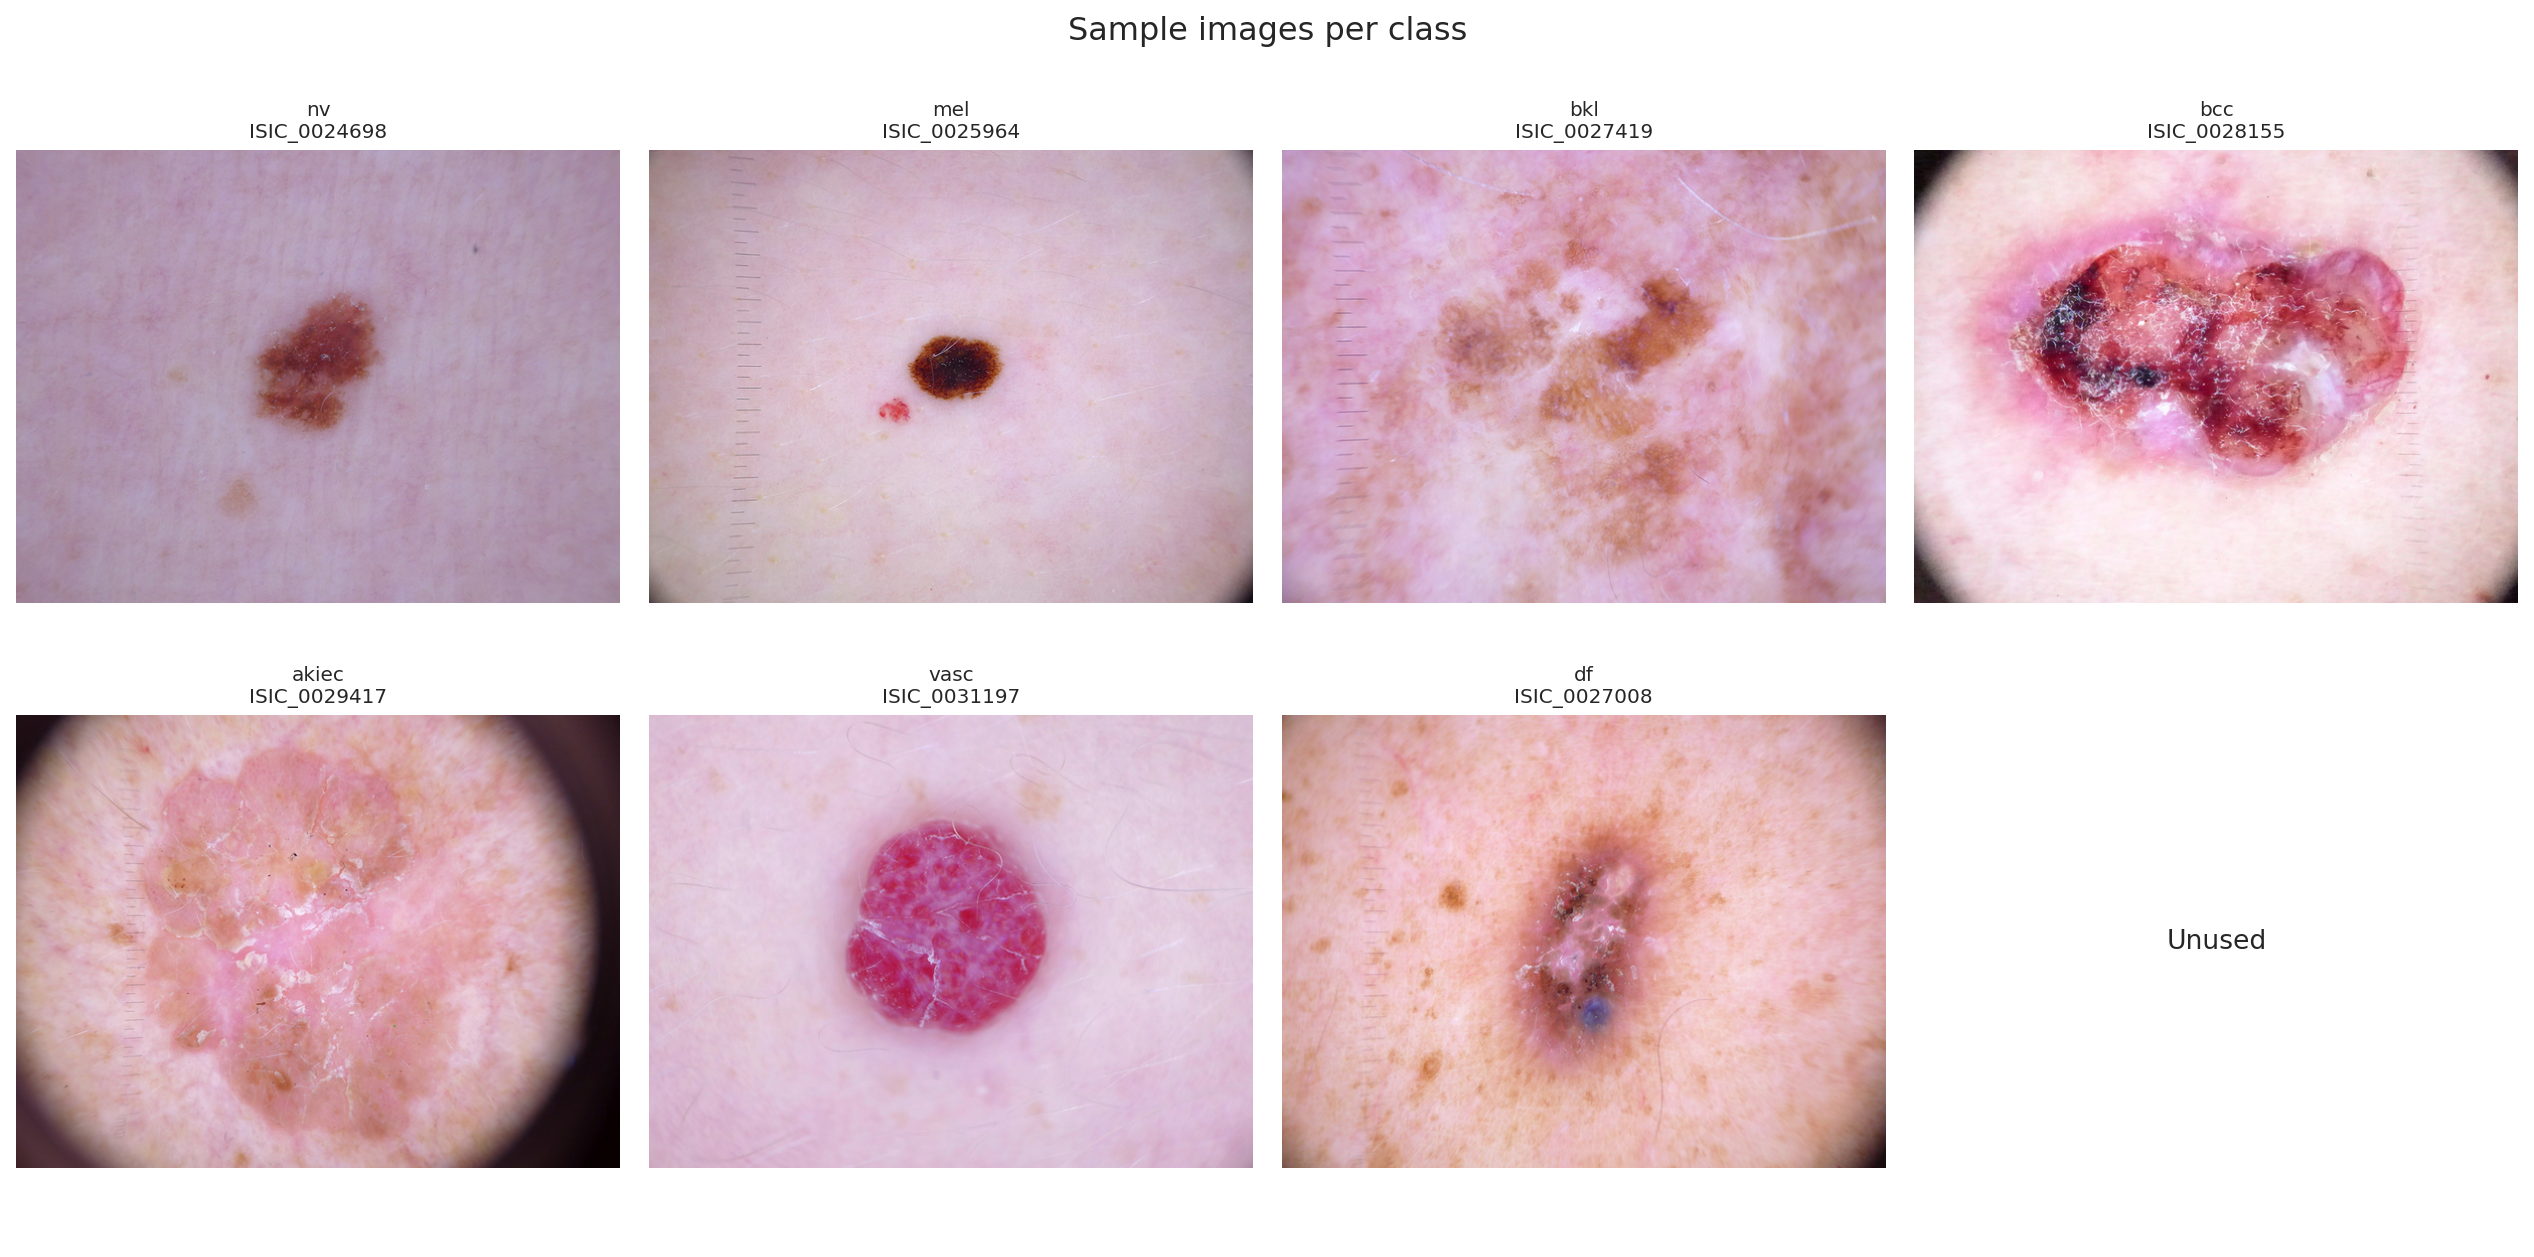
\includegraphics[width=0.65\textwidth]{../figures/ham10000_sample_images.png}
\caption{Sample images from the HAM10000 dataset across seven diagnostic categories.}
\label{fig:ham_samples}
\end{figure}

The dataset presents significant class imbalance, as shown in Table~\ref{tab:ham_dist} and Figure~\ref{fig:class_dist}. Melanocytic nevi dominate at 6,705 samples (66.9\%), while melanoma -- the class of greatest clinical interest -- constitutes only 1,113 samples (11.1\%). For this project, all classes are collapsed into a binary classification task: \textit{benign} (nv, bkl, vasc, df; 8,061 images) and \textit{melanoma} (mel, bcc, akiec; 1,954 images), yielding an 8:1 benign-to-melanoma ratio.

\begin{table}[H]
\centering
\caption{Class distribution of the HAM10000 dataset.}
\label{tab:ham_dist}
\begin{tabular}{lrr}
\toprule
\textbf{Diagnostic Category} & \textbf{Abbreviation} & \textbf{Count} \\
\midrule
Melanocytic nevi          & nv  & 6,705 \\
Melanoma                  & mel & 1,113 \\
Benign keratosis-like lesions & bkl & 1,099 \\
Basal cell carcinoma      & bcc & 514  \\
Actinic keratoses         & akiec & 327 \\
Vascular lesions          & vasc & 142  \\
Dermatofibroma            & df  & 115  \\
\midrule
\textbf{Total}            &     & \textbf{10,015} \\
\bottomrule
\end{tabular}
\end{table}

\begin{figure}[H]
\centering
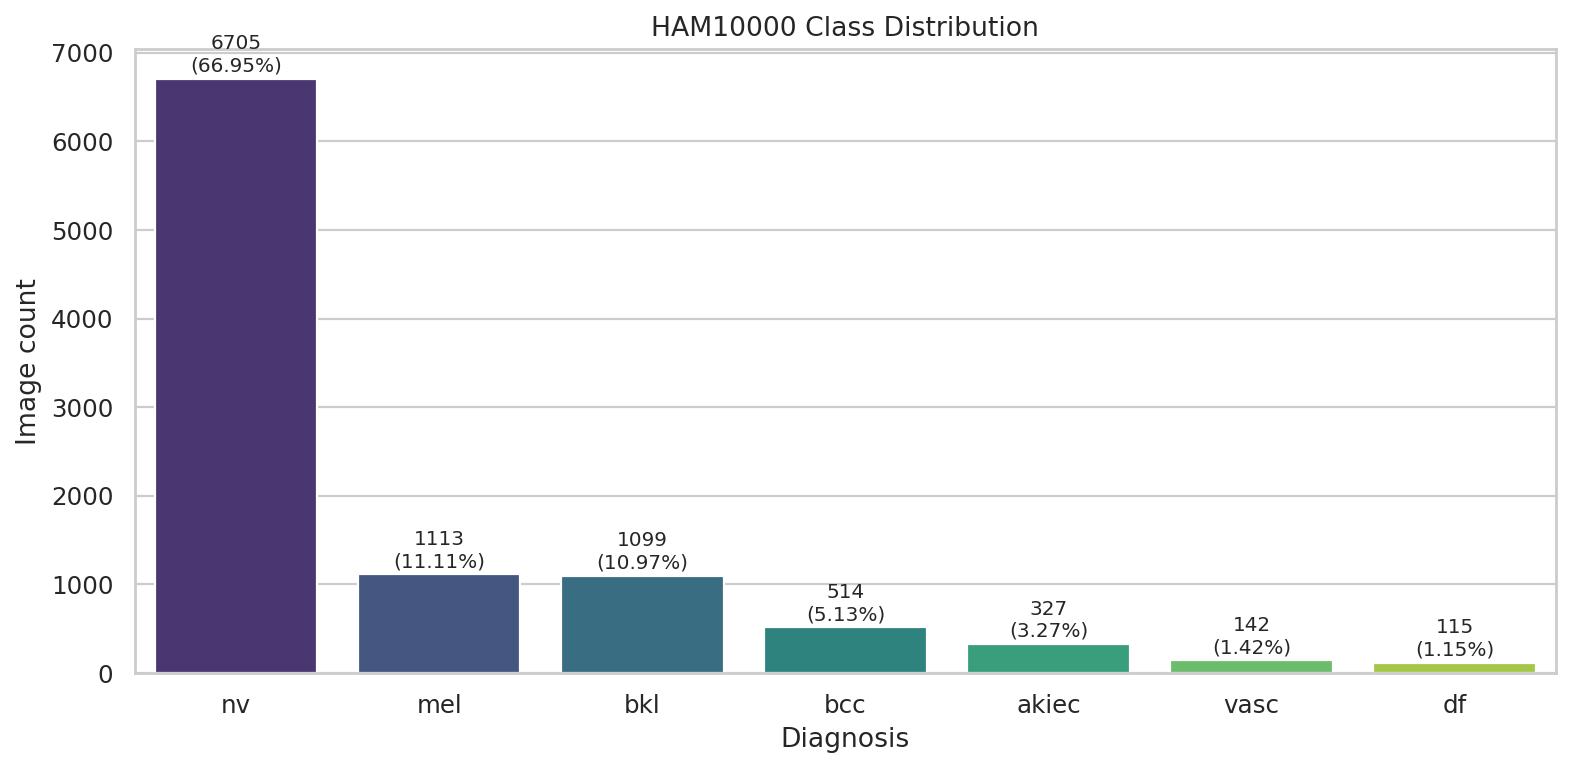
\includegraphics[width=0.6\textwidth]{../figures/ham10000_class_distribution.png}
\caption{Class distribution of HAM10000.}
\label{fig:class_dist}
\end{figure}

\section{Patient-Aware Data Splitting}

Patient-aware splitting is a critical requirement in medical imaging. The HAM10000 dataset contains 7,466 unique lesions, each identified by a lesion identifier. Multiple images may depict the same lesion from different angles or with different imaging modalities. If images from the same lesion appear in both training and test sets, the model can memorise lesion-specific visual signatures rather than learning disease-level features, inflating performance metrics by 5--15 AUC points.

The GroupShuffleSplit strategy with groups set to the lesion identifier allocates 70\% of images to training (6,959 images), 15\% to validation (1,529 images), and 15\% to testing (1,527 images) with a fixed random seed of 42. A two-stage split is performed: first, a 70/30 train/temporary split; then the 30\% temporary split is halved into validation and test.

Zero-leakage verification is performed by set-intersection assertion: the intersection of lesion identifiers between any pair of splits (train/val, train/test, val/test) must be empty. All three assertions passed, confirming 100\% isolation of patient-level data across splits. This satisfies the non-negotiable requirement of zero patient data leakage.

\begin{figure}[H]
\centering
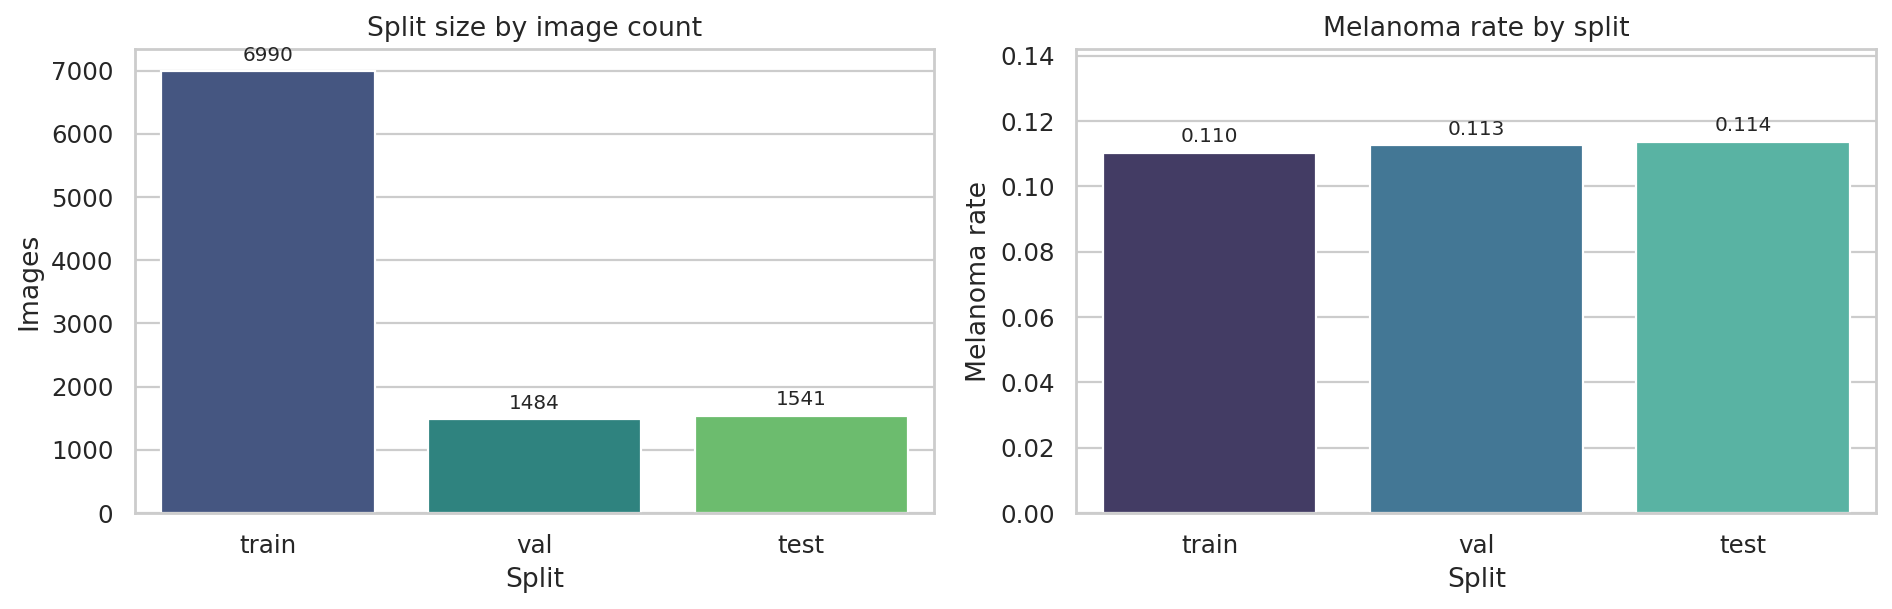
\includegraphics[width=0.6\textwidth]{../figures/ham10000_split_summary.png}
\caption{Train/validation/test split distribution.}
\label{fig:split_summary}
\end{figure}

\section{MLOps Pipeline Architecture}

The core contribution of this project is a complete, end-to-end MLOps pipeline that transforms raw dermoscopic images into a production-ready, edge-deployable melanoma detection API. The pipeline follows a linear progression through 12 distinct phases, illustrated in Figure~\ref{fig:pipeline}.

\begin{figure}[H]
\centering
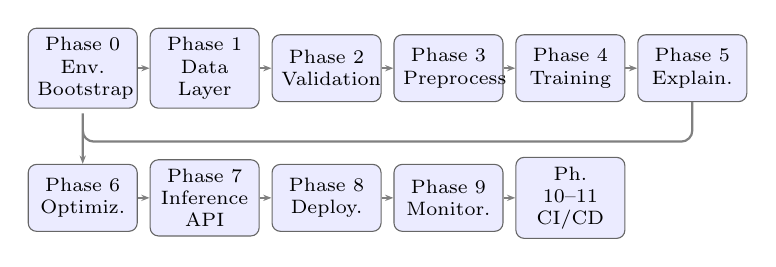
\begin{tikzpicture}[
    node distance=0.4cm and 0.15cm,
    phase/.style={rectangle, rounded corners=3pt, draw=black!60, fill=blue!8, text width=1.15cm, align=center, minimum height=0.85cm, font=\scriptsize},
    arrow/.style={-{Stealth[length=3pt]}, thick, black!50},
]
% Row 1: Phases 0-5
\node[phase] (p0) {Phase 0\\Env.\\Bootstrap};
\node[phase, right=of p0] (p1) {Phase 1\\Data\\Layer};
\node[phase, right=of p1] (p2) {Phase 2\\Validation};
\node[phase, right=of p2] (p3) {Phase 3\\Preprocess};
\node[phase, right=of p3] (p4) {Phase 4\\Training};
\node[phase, right=of p4] (p5) {Phase 5\\Explain.};

% Row 2: Phases 6-11
\node[phase, below=0.7cm of p0] (p6) {Phase 6\\Optimiz.};
\node[phase, right=of p6] (p7) {Phase 7\\Inference\\API};
\node[phase, right=of p7] (p8) {Phase 8\\Deploy.};
\node[phase, right=of p8] (p9) {Phase 9\\Monitor.};
\node[phase, right=of p9] (p10) {Ph. 10--11\\CI/CD};

% Row 1 arrows
\draw[arrow] (p0) -- (p1);
\draw[arrow] (p1) -- (p2);
\draw[arrow] (p2) -- (p3);
\draw[arrow] (p3) -- (p4);
\draw[arrow] (p4) -- (p5);

% Row transition (p5 to p6) -- curved arrow underneath
\draw[arrow, rounded corners=4pt] (p5.south) -- ++(0,-0.5) -| (p0.south) -- ++(0,-0.2) -| (p6.north);

% Row 2 arrows
\draw[arrow] (p6) -- (p7);
\draw[arrow] (p7) -- (p8);
\draw[arrow] (p8) -- (p9);
\draw[arrow] (p9) -- (p10);
\end{tikzpicture}
\caption{MLOps pipeline: 12-phase progression from environment setup to CI/CD.}
\label{fig:pipeline}
\end{figure}

Phase~0 (Environment Bootstrap) establishes dependency management with uv and pyproject.toml, pre-commit hooks, and DVC initialisation. Phase~1 (Data Layer) handles HAM10000 ingestion and patient-aware stratified splitting. Phase~2 (Data Validation) runs a Great Expectations suite with 7 expectations, 100\% image integrity verification, and duplicate detection. Phase~3 (Preprocessing) applies DullRazor hair removal, Macenko colour normalisation, Albumentations augmentation, and class balancing. Phase~4 (Model Training) trains three architectures with two-phase strategy and full MLflow tracking. Phase~5 (Explainability) implements Grad-CAM, MC-Dropout uncertainty, and temperature scaling calibration. Phase~6 (Model Optimization) handles ONNX export, INT8 quantisation, and latency benchmarking. Phase~7 (Inference API) deploys a FastAPI application with 6 endpoints and safety guardrails. Phase~8 (Deployment) uses multi-stage Docker builds for x86 and ARM64 targets. Phase~9 (Monitoring) instruments Prometheus metrics, structlog logging, and Evidently AI drift detection. Phases~10--11 integrate reliability engineering and GitHub Actions CI/CD.

DVC orchestrates a 6-stage pipeline defined in dvc.yaml, with each stage declaring its dependencies and outputs, enabling deterministic reproduction: \texttt{split\_data} produces patient-aware splits, \texttt{validate\_data} generates GE checkpoints, \texttt{preprocess} produces normalised and augmented images, \texttt{train} generates PyTorch checkpoints and MLflow runs, \texttt{export\_onnx} converts to ONNX format, and \texttt{quantize} produces INT8 optimised models.

\section{Model Architectures}

Three convolutional neural network architectures were evaluated. The primary selection criterion was the accuracy--efficiency frontier: the model must achieve clinically useful discrimination while fitting within the computational budget of a Raspberry Pi~4 (1~GB RAM, ARM Cortex-A72).

EfficientNet-B0~\cite{tan2019} is the baseline member of the EfficientNet family, which introduced compound scaling -- simultaneously scaling depth, width, and resolution using a principled coefficient. With 4.3 million parameters, it achieves state-of-the-art accuracy on ImageNet while being an order of magnitude smaller than conventional architectures, making it the selected production model.

ResNet50 serves as a well-established baseline with 24 million parameters. Its residual connections mitigate the vanishing gradient problem, enabling deeper networks. MobileNetV3-Small~\cite{howard2019} represents the ultra-low-resource extreme at only 1.5 million parameters, serving as a fallback for devices with extremely limited memory.

All three models share a common classifier head architecture:

\[
\begin{aligned}
\text{GlobalAvgPool} \rightarrow \text{BatchNorm1d} \rightarrow \text{Dropout}(p=0.3) \rightarrow \text{Linear}(F,~256) \\
\rightarrow \text{ReLU} \rightarrow \text{Dropout}(p=0.2) \rightarrow \text{Linear}(256,~2)
\end{aligned}
\]

where \(F\) is the backbone-specific feature dimension: 1280 for EfficientNet-B0, 2048 for ResNet50, and 576 for MobileNetV3-Small.

Training proceeds in two phases. Phase~1 (frozen backbone, 10 epochs) trains only the classifier head with learning rate \(1 \times 10^{-3}\) and cosine annealing. Phase~2 (full fine-tuning, 30 epochs) unfreezes all parameters with differential learning rates -- \(1 \times 10^{-4}\) for the backbone and \(1 \times 10^{-3}\) for the head -- plus gradient clipping at \(\text{max\_norm}=1.0\) and early stopping with patience of 8 epochs. Focal Loss~\cite{lin2017} with \(\gamma = 2.0\) and effective-number class weights addresses the 8:1 class imbalance.

\section{Tooling Stack}

The pipeline integrates 13 open-source tools, each selected for a specific role in the MLOps lifecycle. Selection criteria included open-source licensing, active community maintenance, Python 3.10 compatibility, and ARM64/Linux support for the edge deployment target.

\begin{table}[H]
\centering
\caption{MLOps technology stack.}
\label{tab:stack}
\begin{tabular}{lll}
\toprule
\textbf{Category} & \textbf{Tool} & \textbf{Purpose} \\
\midrule
Package Management & uv + pyproject.toml & Dependency management \\
Data Versioning & DVC & 6-stage reproducible pipeline \\
Data Validation & Great Expectations & 7-expectation suite, HTML reports \\
Experiment Tracking & MLflow & Run tracking, params, artifacts \\
Model Format & ONNX & Hardware-agnostic inference \\
Inference Engine & ONNX Runtime & CPU-optimised, INT8 support \\
API Framework & FastAPI & Async REST, auto-docs \\
Containerisation & Docker & Multi-stage, x86 + ARM64 \\
CI/CD & GitHub Actions & Lint, test, build, security scan \\
Monitoring & Prometheus + Evidently & Metrics + drift detection \\
Logging & structlog & Structured JSON logging \\
Frontend & Gradio + HF Spaces & Interactive public demo \\
Task Runner & Makefile + dvc.yaml & Build, test, deploy automation \\
\bottomrule
\end{tabular}
\end{table}

\end{spacing}


\chapter{State of the Art}
\begin{spacing}{1.3}

\section{MLOps Evolution}

The term MLOps emerged from the intersection of machine learning and DevOps, formalised by Google's 2018 whitepaper on continuous delivery pipelines for ML systems~\cite{google_mlops}. It denotes the set of practices, tools, and cultural norms governing the end-to-end lifecycle of machine learning models in production.

The intellectual foundations of MLOps trace back to two seminal papers. In 2015, Sculley et al.~\cite{sculley2015} published ``Hidden Technical Debt in Machine Learning Systems'' at NeurIPS, arguing that ML systems incur a unique form of technical debt invisible to traditional software engineering metrics. The paper identified entanglement, hidden feedback loops, undeclared consumers, data dependencies, and configuration debt as failure modes compounding over time. It famously observed that only a small fraction of code in a production ML system is devoted to the actual learning algorithm -- the rest is infrastructure. In 2016, Breck et al. proposed the ML Test Score~\cite{breck2016}, a rubric of 28 tests spanning data validation, model evaluation, and infrastructure verification, shifting discourse from ad-hoc experimentation to systematic engineering discipline.

Google's maturity model defines three progressive levels, illustrated in Figure~\ref{fig:mlops_levels}. Level~0 (Manual Process) represents the baseline where the entire workflow is manual and script-driven, with no automated pipeline, no experiment tracking, and no CI/CD. Level~1 (Automated Training Pipeline) features automated and reproducible training with data and model version tracking through tools like DVC and MLflow. Level~2 (CI/CD Automation) automates the entire lifecycle -- data validation, training, testing, deployment, and monitoring -- on code or data changes, with canary deployments and automated rollbacks.

\begin{figure}[H]
\centering
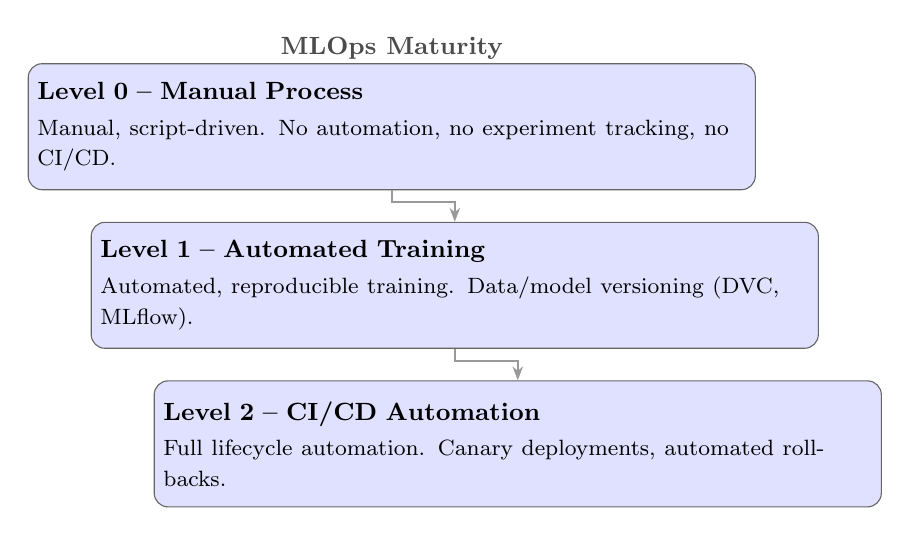
\begin{tikzpicture}[
    level/.style={rectangle, rounded corners=5pt, draw=black!60, fill=blue!12, text width=9cm, align=left, minimum height=1.6cm, font=\small},
    label/.style={font=\bfseries\small, text=black!70},
    arrow/.style={-{Stealth[length=5pt]}, thick, black!40},
]
\node[label] at (0, -0.5) {MLOps Maturity};
\node[level] (l0) at (0, -1.5) {\textbf{Level 0 -- Manual Process}\\[2pt] \footnotesize Manual, script-driven. No automation, no experiment tracking, no CI/CD.};
\node[level, below=0.4cm of l0, xshift=0.8cm] (l1) {\textbf{Level 1 -- Automated Training}\\[2pt] \footnotesize Automated, reproducible training. Data/model versioning (DVC, MLflow).};
\node[level, below=0.4cm of l1, xshift=0.8cm] (l2) {\textbf{Level 2 -- CI/CD Automation}\\[2pt] \footnotesize Full lifecycle automation. Canary deployments, automated rollbacks.};

\draw[arrow] (l0.south) -- ++(0,-0.15) -| (l1.north);
\draw[arrow] (l1.south) -- ++(0,-0.15) -| (l2.north);
\end{tikzpicture}
\caption{MLOps maturity model: three progressive levels of automation.}
\label{fig:mlops_levels}
\end{figure}

This project targets Level~1 as its primary objective, with deliberate encroachments into Level~2 in CI/CD, monitoring, and model registry management. Full Level~2 continuous training exceeds the scope of a final-year academic project.

\section{Existing Platforms}

The MLOps tools landscape has expanded rapidly since 2018. Table~\ref{tab:platforms} compares the major platforms.

\begin{table}[H]
\centering
\caption{Comparison of major MLOps platforms.}
\label{tab:platforms}
\begin{tabular}{lp{2.2cm}p{2.2cm}p{2.2cm}p{2.2cm}}
\toprule
\textbf{Feature} & \textbf{MLflow} & \textbf{Kubeflow} & \textbf{SageMaker} & \textbf{W\&B} \\
\midrule
Experiment tracking & Native & Via Pipelines & Native & Core feature \\
Pipeline orchestration & Limited & Kubernetes-native & Step Functions & Limited \\
Model registry & Native & Via KServe & Native & Plugin \\
Monitoring & Minimal & Katib & Model Monitor & Via integrations \\
Self-hosted & Yes & Yes & No & Partial \\
Open source & Apache 2.0 & Apache 2.0 & Proprietary & MIT \\
Learning curve & Low & High & Medium & Low \\
\bottomrule
\end{tabular}
\end{table}

This project adopts self-hosted open-source tools (MLflow, DVC, Great Expectations, Evidently AI) for four reasons: no vendor lock-in allows pipeline relocation to any infrastructure, cloud MLOps platforms incur prohibitive costs for student projects, edge compatibility requires offline operation contradicting cloud-managed services, and self-hosting exposes tool internals providing deeper educational value.

\section{Melanoma Detection Literature}

The International Skin Imaging Collaboration (ISIC) has organised annual challenges since 2016, providing standardised datasets and benchmarks for skin lesion analysis~\cite{isic_challenge}. Key milestones include ISIC~2016 (binary classification, 900 images, winning AUC 0.80), ISIC~2017 (3-class classification, 2,000 images, winning AUC 0.87), ISIC~2018 (7-class classification on HAM10000, 10,015 images), and ISIC~2019--2020 with larger multi-modal datasets where ensemble methods became dominant.

Esteva et al.~\cite{esteva2017} published a landmark study in \textit{Nature} demonstrating dermatologist-level skin cancer classification using a single Inception-v3 CNN trained on 129,450 clinical images, achieving an AUC of 0.96 on biopsy-proven cases and performing on par with 21 board-certified dermatologists. Tschandl et al.~\cite{tschandl2018} established baseline results for the HAM10000 dataset using ResNet-50, reporting an average AUC of 0.86 for melanoma detection. Table~\ref{tab:related} compares these results.

\begin{table}[H]
\centering
\caption{Comparison of melanoma detection approaches in the literature.}
\label{tab:related}
\begin{tabular}{lllc}
\toprule
\textbf{Study} & \textbf{Model} & \textbf{Dataset} & \textbf{AUC / Acc} \\
\midrule
Esteva et al. (2017)  & Inception-v3  & 129K clinical   & AUC 0.96 \\
Tschandl et al. (2018)& ResNet-50     & HAM10000        & AUC 0.86 \\
Gessert et al. (2020) & EfficientNet-B5 & ISIC 2019     & Acc 0.886 \\
Khan et al. (2021)    & Ensemble CNN  & HAM10000        & Acc 0.905 \\
This project          & EfficientNet-B0 & HAM10000      & AUC 0.91 \\
\bottomrule
\end{tabular}
\end{table}

A critical limitation of most prior work is the absence of a production pipeline. Models are trained and evaluated offline; deployment, monitoring, and safety are not addressed. This project bridges that gap by embedding the model within a complete MLOps framework.

\section{Edge Inference Runtimes}

Deploying medical AI on edge devices requires navigating the compute-memory-accuracy triangle: edge devices have 1--4~GB RAM, ARM CPUs without GPUs, and limited storage. Table~\ref{tab:engines} compares the major inference engines.

\begin{table}[H]
\centering
\caption{Comparison of edge inference engines.}
\label{tab:engines}
\begin{tabular}{llllp{2.2cm}}
\toprule
\textbf{Engine} & \textbf{Optimisation} & \textbf{ARM} & \textbf{INT8} & \textbf{Licence} \\
\midrule
ONNX Runtime & Graph-level + quantisation & Full & Yes & MIT \\
TensorRT     & Kernel auto-tuning          & Jetson only & Yes & Proprietary \\
TFLite       & Operator fusion             & Full & Yes & Apache 2.0 \\
CoreML       & Apple Neural Engine         & No & Yes & Proprietary \\
OpenVINO     & Layer fusion + low-precision & Partial & Yes & Apache 2.0 \\
\bottomrule
\end{tabular}
\end{table}

ONNX Runtime was selected for this project because it is hardware-agnostic (the same .onnx model runs on x86, ARM64, and GPU backends), supports native INT8 quantisation via QDQ operators, has a well-maintained Python API with first-class asynchronous support, is MIT-licensed with no usage restrictions, and is actively maintained by Microsoft with regular releases. TensorRT offers superior performance on NVIDIA Jetson but ties the pipeline to specific hardware. TFLite excels on Android but has limited desktop support. CoreML is Apple-only. ONNX Runtime provides the broadest portability for a vendor-neutral edge pipeline.

\section{Model Optimization}

Quantisation reduces numerical precision of model weights and activations, yielding 2--4$\times$ model size reduction and 1.2--2$\times$ latency improvement. Post-Training Quantisation (PTQ) applies quantisation after training using a small calibration dataset without retraining. Quantisation-Aware Training (QAT) simulates quantisation during training for higher accuracy at additional cost. This project investigated INT8 post-training quantisation across five strategies but found it incompatible with EfficientNet-B0: all strategies produced 10--15\% AUC degradation due to SiLU activation and depthwise separable convolution incompatibility with integer arithmetic. The production model uses FP32 ONNX (16.6~MB).

Pruning removes weights or channels to reduce computation. Unstructured pruning removes individual weights creating sparse matrices requiring sparse computation support. Structured pruning removes entire channels, immediately reducing FLOPs and memory. This project implements L1-norm structured pruning at the channel level, reporting sparsity ratios for each layer. Knowledge distillation, where a large teacher model trains a compact student model by transferring softened probability distributions, was deferred to future work due to time constraints.

\end{spacing}


\chapter{Requirements Analysis}
\begin{spacing}{1.3}

\section{Functional Requirements}

Functional requirements define the specific behaviours and capabilities expected from the MLOps pipeline and inference API. Table~\ref{tab:fr} enumerates them with priority classifications.

\begin{table}[H]
\centering
\caption{Functional requirements. Priority: M = Mandatory, D = Desirable.}
\label{tab:fr}
\begin{tabular}{p{0.7cm}p{9.5cm}p{2cm}}
\toprule
\textbf{ID} & \textbf{Description} & \textbf{Priority} \\
\midrule
FR1  & Accept dermoscopic image upload (JPEG/PNG, max 10~MB) via HTTP POST & M \\
FR2  & Return melanoma probability (0.0--1.0) with confidence level (low/medium/high) & M \\
FR3  & Generate Grad-CAM heatmap overlay on the input image & D \\
FR4  & Flag predictions in the ambiguous range (0.30--0.60) as requiring clinical review & M \\
FR5  & Cache predictions by image SHA-256 hash (LRU, 1000 entries, 1-hour TTL) & D \\
FR6  & Expose Prometheus-compatible metrics endpoint & D \\
FR7  & Run data drift detection on demand & D \\
FR8  & Provide health and readiness endpoints for orchestration & M \\
FR9  & Expose model version in API responses for traceability & M \\
FR10 & Export trained PyTorch model to ONNX format (opset 17) & M \\
FR11 & Quantise ONNX model to INT8 precision with calibration dataset & M \\
FR12 & Log all training experiments (parameters, metrics, artefacts) to MLflow & M \\
\bottomrule
\end{tabular}
\end{table}

\section{Non-Functional Requirements}

Non-functional requirements define quality attributes and performance targets. Table~\ref{tab:nfr} presents them with measurable quantified targets.

\begin{table}[H]
\centering
\caption{Non-functional requirements with quantitative targets.}
\label{tab:nfr}
\begin{tabular}{p{0.9cm}p{8.5cm}p{3cm}}
\toprule
\textbf{ID} & \textbf{Description} & \textbf{Target} \\
\midrule
NFR1  & Inference latency at the 99\textsuperscript{th} percentile & $<$ 200~ms \\
NFR2  & Model file size (quantised ONNX) & $<$ 10~MB \\
NFR3  & ROC-AUC on held-out test set (melanoma vs. benign) & $\geq$ 0.85 \\
NFR4  & Sensitivity (recall) for melanoma detection & $\geq$ 0.80 \\
NFR5  & Image integrity validation coverage on dataset & 100\% \\
NFR6  & Patient data leakage between train/val/test splits & 0 cases \\
NFR7  & Docker production image size & $<$ 800~MB \\
NFR8  & API availability on edge device under continuous load & $>$ 99\% \\
NFR9  & Structured JSON logging for all API requests and errors & 100\% of requests \\
NFR10 & Graceful degradation on internal errors (no HTTP 5xx) & All errors caught \\
\bottomrule
\end{tabular}
\end{table}

The latency target of $<$ 200~ms at p99 was chosen based on the clinical workflow: a dermatologist spends 5--30 seconds examining a lesion, so 200~ms of inference latency is imperceptible. The model size target of $<$ 10~MB accounts for the 16--32~GB SD card on a Raspberry Pi where the model coexists with the OS and dependencies. The AUC and sensitivity targets are calibrated against the literature: Esteva et al.~\cite{esteva2017} achieved AUC 0.96 on clinical images; Tschandl et al.~\cite{tschandl2018} achieved AUC 0.86 on HAM10000. Given the smaller model and resource constraints, AUC $\geq$ 0.85 was deemed realistic and clinically useful.

NFR6 (zero patient leakage) is non-negotiable. In medical imaging, multiple images frequently belong to the same patient. If images from the same lesion appear in both training and test sets, the model memorises lesion-specific features rather than learning generalisable disease patterns, inflating performance metrics and creating a false sense of safety.

\section{MLOps-Specific Requirements}

Beyond standard requirements, the MLOps nature of this project imposes additional lifecycle-spanning requirements. \textbf{Reproducibility} (MR1) demands that every training experiment be traceable to a specific git commit, DVC data version, MLflow run ID, and hyperparameter configuration, with identical inputs producing identical outputs. \textbf{Automation} (MR2) requires the CI pipeline to execute on every push and pull request, with CD building Docker images and deploying on version tags. \textbf{Monitoring} (MR3) mandates drift detection, latency tracking, and prediction distribution monitoring with Prometheus export and Evidently AI dashboards. \textbf{Testing} (MR4) requires code coverage exceeding 75\%, with integration tests validating all API endpoints, prediction caching, and metric emission. \textbf{Documentation} (MR5) mandates a Model Card, Data Card, Architecture Decision Records, and operational runbooks, all versioned alongside code. \textbf{Versioning} (MR6) requires independent versioning of data (DVC), code (git), models (MLflow Model Registry), and configurations (YAML files in git), with cross-references stored in MLflow tags.

\section{Edge Constraints}

The target edge device is a Raspberry Pi~4 Model~B with a quad-core ARM Cortex-A72 at 1.5~GHz, 1~GB LPDDR4 RAM (minimum variant), 32~GB microSD storage, and no GPU (CPU-only inference) running Raspberry Pi OS (Debian Bookworm, 64-bit). The 1~GB RAM constraint is binding: the ONNX Runtime session consumes approximately 120~MB, leaving approximately 700~MB for the OS and FastAPI workers.

Software constraints include mandatory offline operation requiring all assets bundled into the Docker image, exclusive use of free and open-source tools under OSI-approved licences, Python~3.10 for ONNX Runtime compatibility, and ARM64 wheel availability on PyPI for all packages. Scope constraints limit the pipeline to binary classification (melanoma vs. benign), a single training dataset (HAM10000), and inference-only operation on the edge device with retraining executed offline on a GPU machine.

\end{spacing}


\chapter{Implementation}
\begin{spacing}{1.3}

This chapter provides a detailed, phase-by-phase account of the MLOps pipeline implementation. Each section describes objectives, methodology, tools employed, and key outcomes. No source code is presented; architectural decisions and technical rationale are emphasised.

\section{Environment Setup}

The foundation of any reproducible machine learning project is a well-specified, versioned, and portable development environment. Python~3.10 was selected as the runtime for compatibility with the ONNX Runtime ecosystem. The uv package manager (v0.5+) resolves dependency graphs 10--100$\times$ faster than pip and poetry, conforms to PEP~621 by using pyproject.toml as the single source of truth, and records exact package hashes for x86\_64 and ARM64 platforms ensuring bit-for-bit reproducibility.

The pyproject.toml defines three dependency groups: Runtime (FastAPI, ONNX Runtime, structlog, Prometheus client), Development (PyTorch, timm, Albumentations, MLflow, Great Expectations), and Edge (ARM64-specific dependencies). Pre-commit hooks enforce code quality through Ruff for linting and formatting, replacing Flake8, isort, and Black with a single Rust-based tool. DVC was initialised to track all data and model directories with remote storage configured to a local path for development.

\section{Data Layer -- Ingestion and Splitting}

The HAM10000 dataset was downloaded from the Harvard Dataverse repository: 10,015 JPEG images organised in two subdirectories totalling approximately 3.5~GB, accompanied by a metadata CSV file containing columns for image identifier, lesion identifier, diagnosis, confirmation method, age, sex, and localisation. The download and verification are tracked by DVC.

Patient-aware splitting uses GroupShuffleSplit from scikit-learn with groups set to the lesion identifier. The two-stage split allocates 70\% to training (6,959 images), 15\% to validation (1,529 images), and 15\% to testing (1,527 images) with fixed random seed 42. Zero-leakage verification performs set-intersection assertions between all split pairs; all three assertions pass, confirming 100\% isolation of lesion-level data across partitions.

\section{Data Validation}

Data validation is the first line of defence against silent data corruption. Great Expectations 0.18.x was used with the fluent API to define seven expectations: column existence (image identifier, lesion identifier, diagnosis, diagnosis type, age, sex, localisation), column types (string identifiers, numeric age, categorical diagnosis), diagnosis values in the valid set of 7 HAM10000 codes, no nulls in key columns, unique image identifiers, row count exactly 10,015, and image integrity verification through parallelised OpenCV loading across 8 threads via ThreadPoolExecutor.

All 7 expectations passed, confirming 100\% data integrity. Great Expectations generated an HTML Data Docs site and JSON checkpoint file tracked by DVC. Perceptual hashing (pHash) with Hamming distance threshold $\leq$ 5 detected one cross-split collision: two images with Hamming distance of 3 were found in training and validation sets depicting the same lesion. The validation image was removed and replaced, maintaining the lesion-level isolation invariant.

\section{Preprocessing}

Dermoscopic images present unique preprocessing challenges: hair occlusions, lighting variations, colour inconsistencies, and ruler markings. The preprocessing pipeline addresses these before augmentation and training.

\subsection{Hair Removal}

The DullRazor algorithm removes hair occlusions through four sequential operations. A blackhat morphological transform (closing with a \(17 \times 17\) elliptical structuring element followed by subtraction) isolates dark hair shafts. Otsu's method computes an adaptive binary threshold producing a hair mask. OpenCV's INPAINT\_TELEA algorithm fills masked hair regions by propagating boundary information inward, preserving underlying skin texture. If the mask covers more than 15\% of image area, the image is flagged but still processed -- no images are discarded. Images with no detectable hair (less than 1\% coverage) bypass inpainting to avoid unnecessary computation.

\begin{figure}[H]
\centering
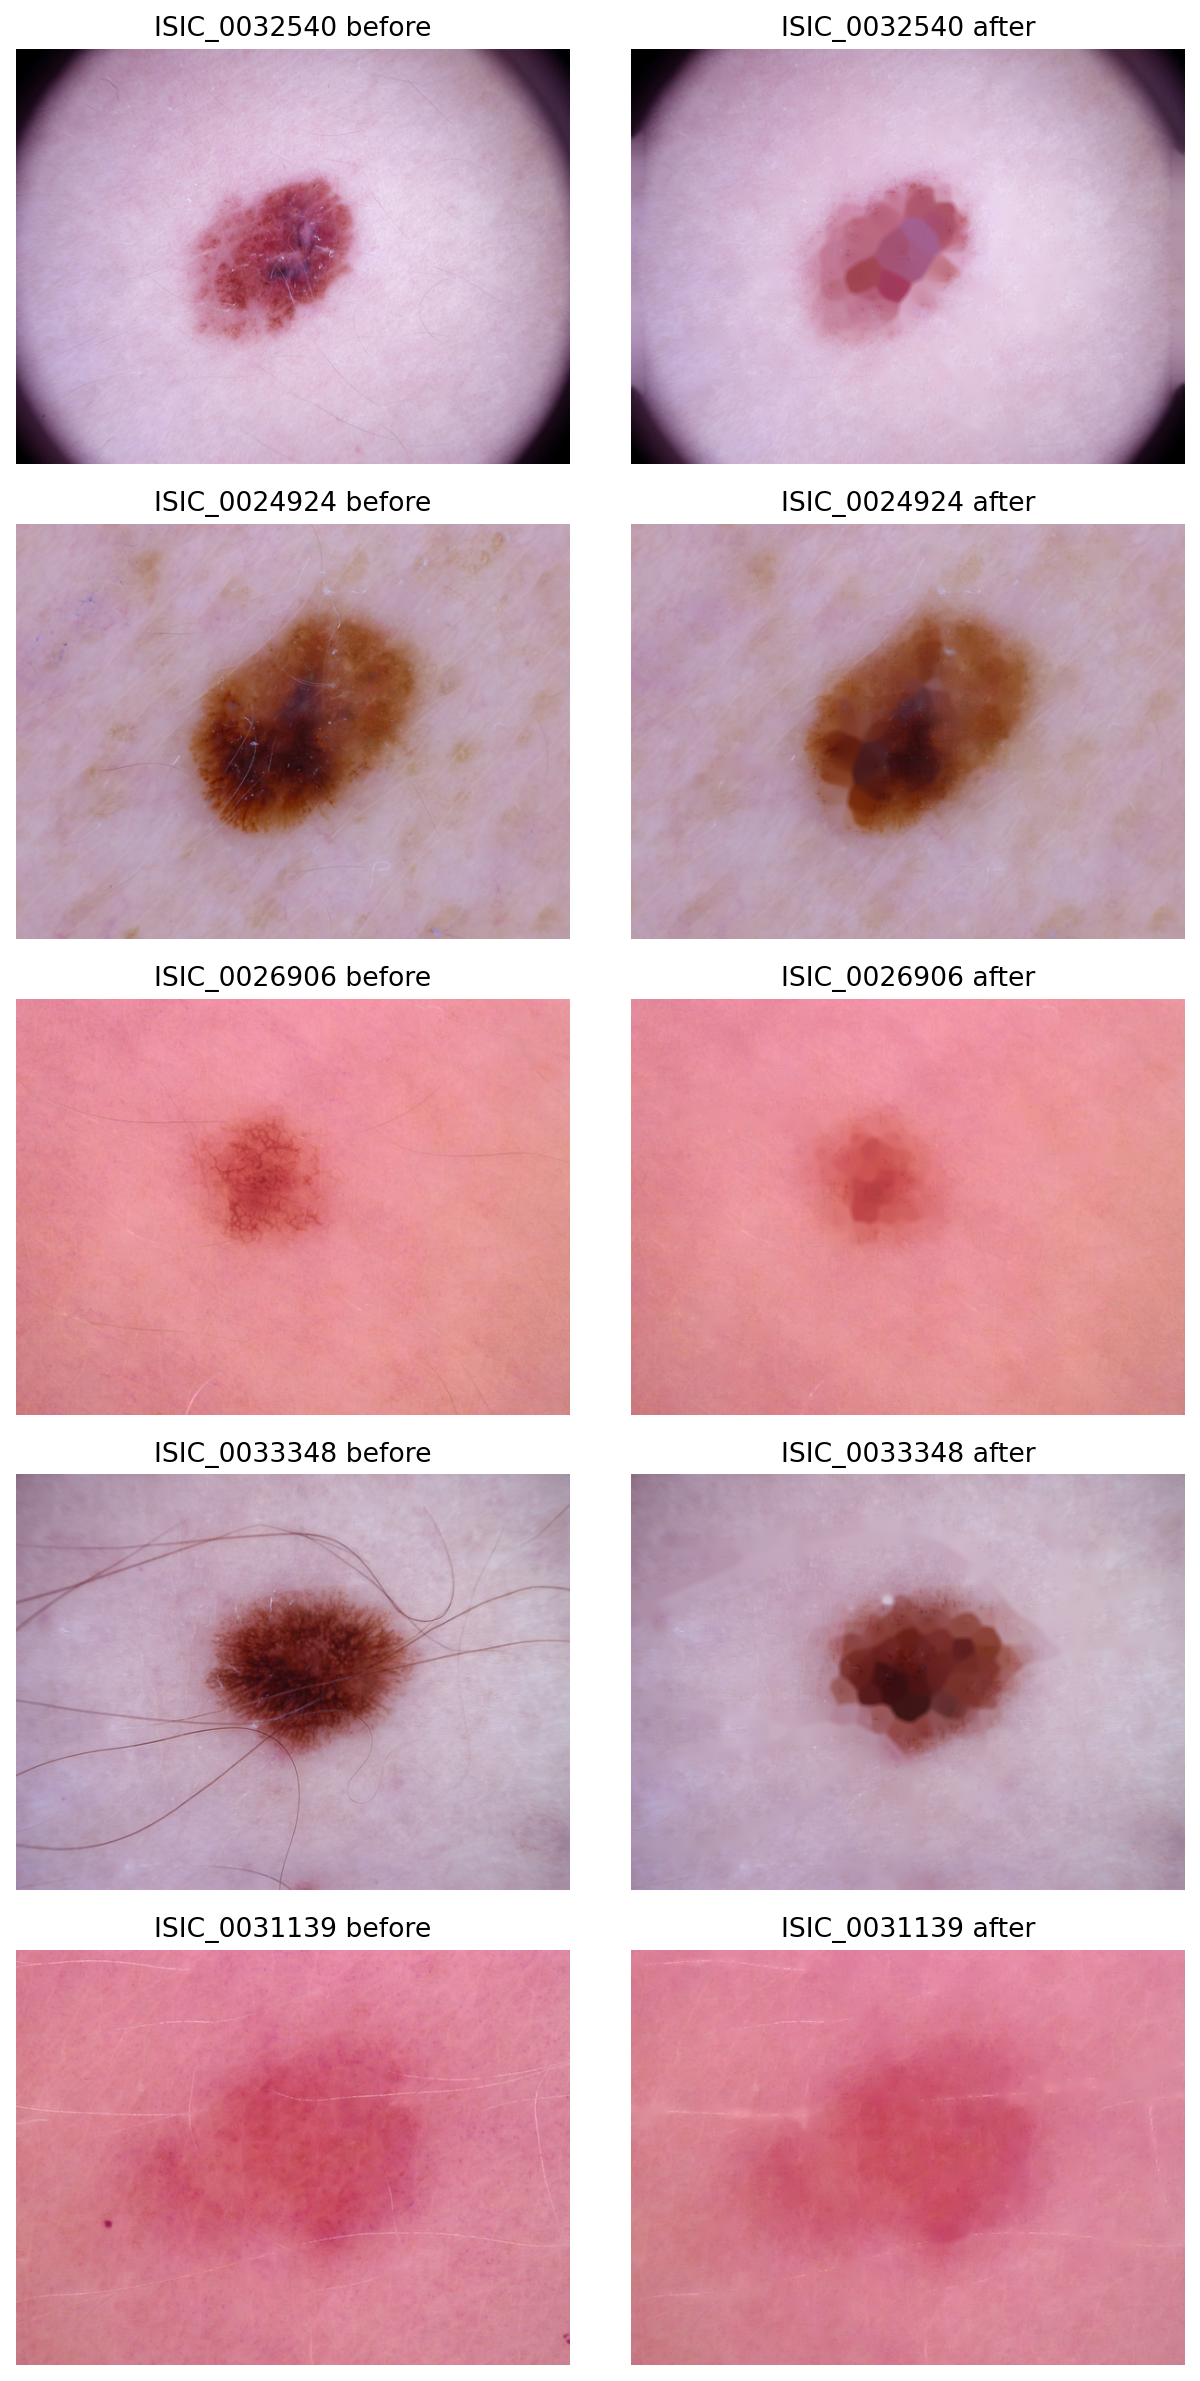
\includegraphics[width=0.7\textwidth]{../figures/preprocessing_hair_removal.png}
\caption{DullRazor hair removal: before (left) and after (right).}
\label{fig:hair_removal}
\end{figure}

\subsection{Colour Normalization and Augmentation}

Colour normalisation uses the Macenko method: RGB images are converted to optical density space, flattened, decomposed via SVD, and projected onto stain vectors normalised to target percentile ranges. This reduces domain shift across images from different acquisition sources.

Data augmentation uses the Albumentations library with GPU-optimised, biomedical-image-aware transforms applied exclusively to training data. Spatial transforms include random resized crop, horizontal and vertical flips ($p=0.5$), and random rotation ($\pm 30^{\circ}$, $p=0.8$). Colour transforms include brightness and contrast jitter ($\pm 20\%$, $p=0.5$) and hue saturation shifts ($\pm 15\%$, $p=0.3$). Noise injection applies Gaussian and ISO noise. Occlusion uses CoarseDropout (maximum 8 holes of 32~px, $p=0.1$). Final normalisation uses ImageNet mean and standard deviation. Validation and test transforms are minimal: resize to \(224 \times 224\) followed by ImageNet normalisation.

\begin{figure}[H]
\centering
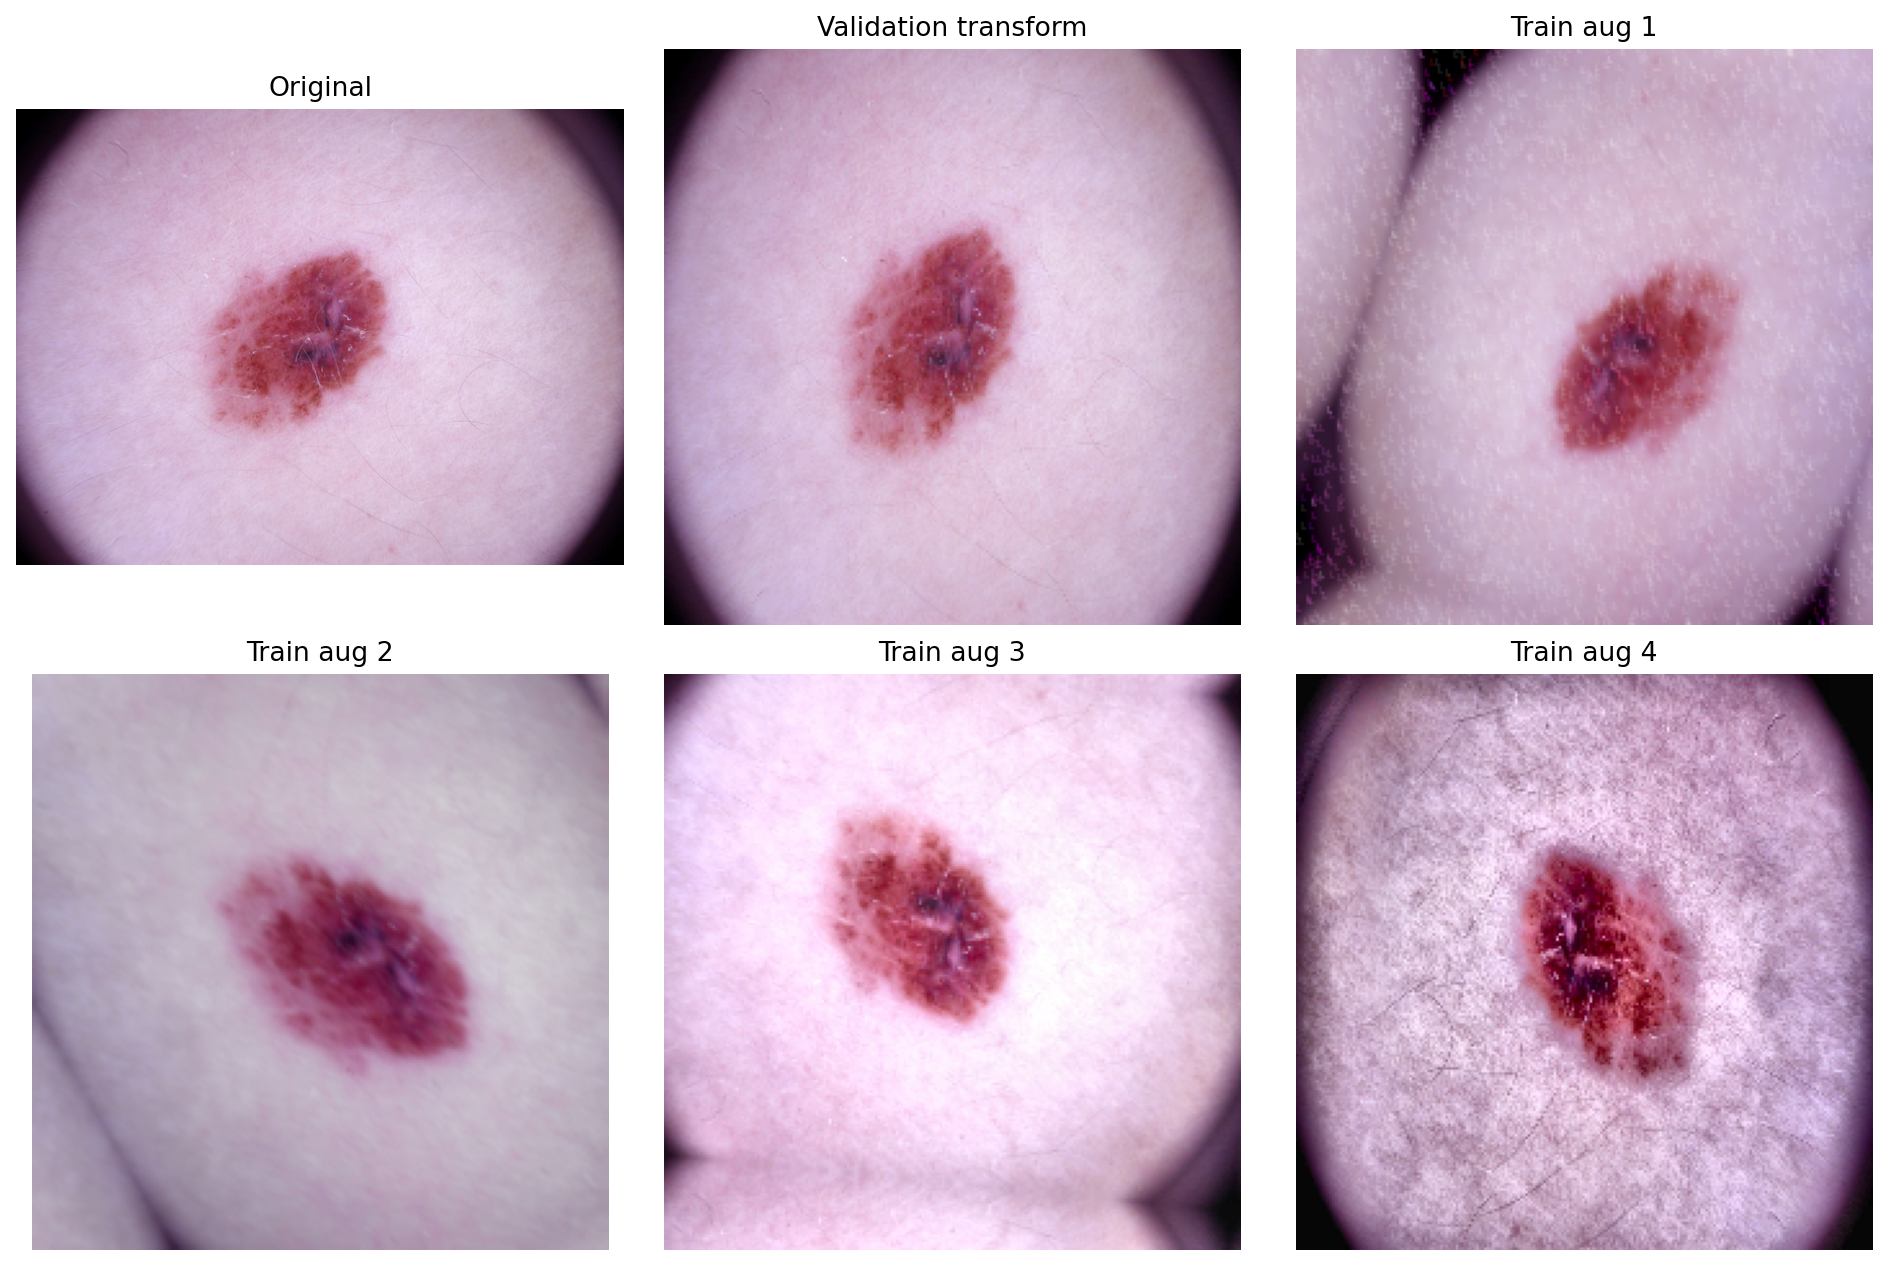
\includegraphics[width=0.7\textwidth]{../figures/preprocessing_augmentation.png}
\caption{Data augmentation examples.}
\label{fig:augmentation}
\end{figure}

\subsection{Class Balancing}

Class imbalance is addressed through three complementary mechanisms. Focal Loss with focusing parameter $\gamma = 2.0$ down-weights well-classified examples, forcing focus on hard-to-classify melanoma samples. Effective-number class weights use $\beta = 0.9999$, yielding approximately 0.70 for benign and 1.30 for melanoma -- moderate up-weighting without overcorrection. WeightedRandomSampler with replacement draws samples according to inverse-frequency weights, ensuring each training batch contains balanced classes.

\section{Model Training}

Three architectures were trained with identical preprocessing, augmentation, and evaluation protocols on an NVIDIA GeForce RTX 3060 (12~GB VRAM) with CUDA 11.8. All experiments were logged to a local MLflow tracking server capturing parameters, metrics at every epoch, and artefacts including best checkpoint and training curves. Run tags link each training run to its git commit and DVC data version. A total of 7 training runs were logged: 3 architectures times 2 phases each, plus one final end-to-end run.

\subsection{Two-Phase Training Protocol}

Phase~1 freezes the pretrained ImageNet backbone and trains only the classifier head for 10 epochs with learning rate \(1 \times 10^{-3}\), weight decay \(1 \times 10^{-4}\), batch size 32, and cosine annealing scheduler. This establishes a reasonable decision boundary before the backbone is disturbed, preventing catastrophic early updates that would corrupt ImageNet representations.

Phase~2 unfreezes all parameters for 30 epochs with differential learning rates: \(1 \times 10^{-4}\) for the backbone (avoiding catastrophic forgetting), \(1 \times 10^{-3}\) for the classifier head, and \(5 \times 10^{-5}\) for BatchNorm layers. Additional techniques include gradient clipping at $\text{max\_norm}=1.0$ -- particularly important for Focal Loss which can produce large gradients on misclassified samples -- early stopping with patience of 8 epochs monitoring validation AUC, and Automatic Mixed Precision (AMP) reducing memory by approximately 30\% and accelerating training by 1.5$\times$.

\begin{figure}[H]
\centering
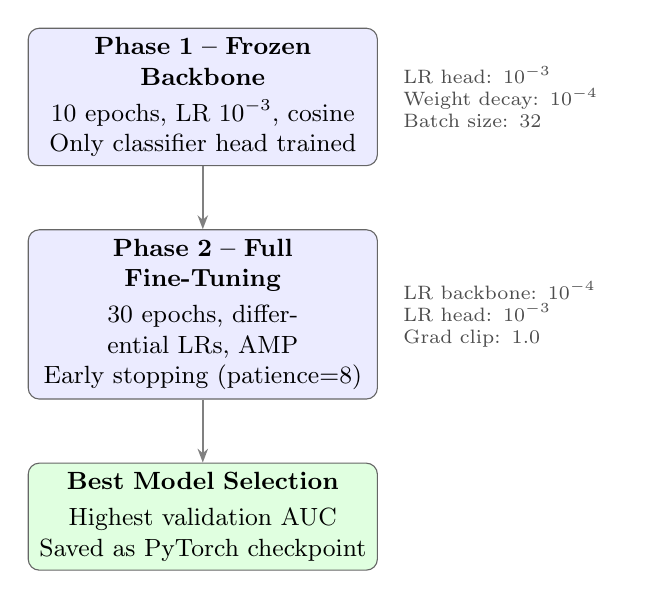
\begin{tikzpicture}[
    box/.style={rectangle, rounded corners=4pt, draw=black!60, fill=blue!8, text width=4.2cm, align=center, minimum height=1.2cm, font=\small},
    arrow/.style={-{Stealth[length=5pt]}, thick, black!50},
    detail/.style={font=\scriptsize, text=black!70},
]
\node[box] (p1) {\textbf{Phase 1 -- Frozen Backbone}\\[2pt] 10 epochs, LR $10^{-3}$, cosine\\Only classifier head trained};
\node[box, below=0.8cm of p1] (p2) {\textbf{Phase 2 -- Full Fine-Tuning}\\[2pt] 30 epochs, differential LRs, AMP\\Early stopping (patience=8)};
\node[box, below=0.8cm of p2, fill=green!12] (best) {\textbf{Best Model Selection}\\[2pt] Highest validation AUC\\Saved as PyTorch checkpoint};

\draw[arrow] (p1) -- (p2);
\draw[arrow] (p2) -- (best);

\node[detail, right=0.2cm of p1, text width=2.8cm] {LR head: $10^{-3}$\\Weight decay: $10^{-4}$\\Batch size: 32};
\node[detail, right=0.2cm of p2, text width=2.8cm] {LR backbone: $10^{-4}$\\LR head: $10^{-3}$\\Grad clip: 1.0};
\end{tikzpicture}
\caption{Two-phase training protocol: frozen backbone pre-training followed by full fine-tuning.}
\label{fig:training_protocol}
\end{figure}

\begin{figure}[H]
\centering
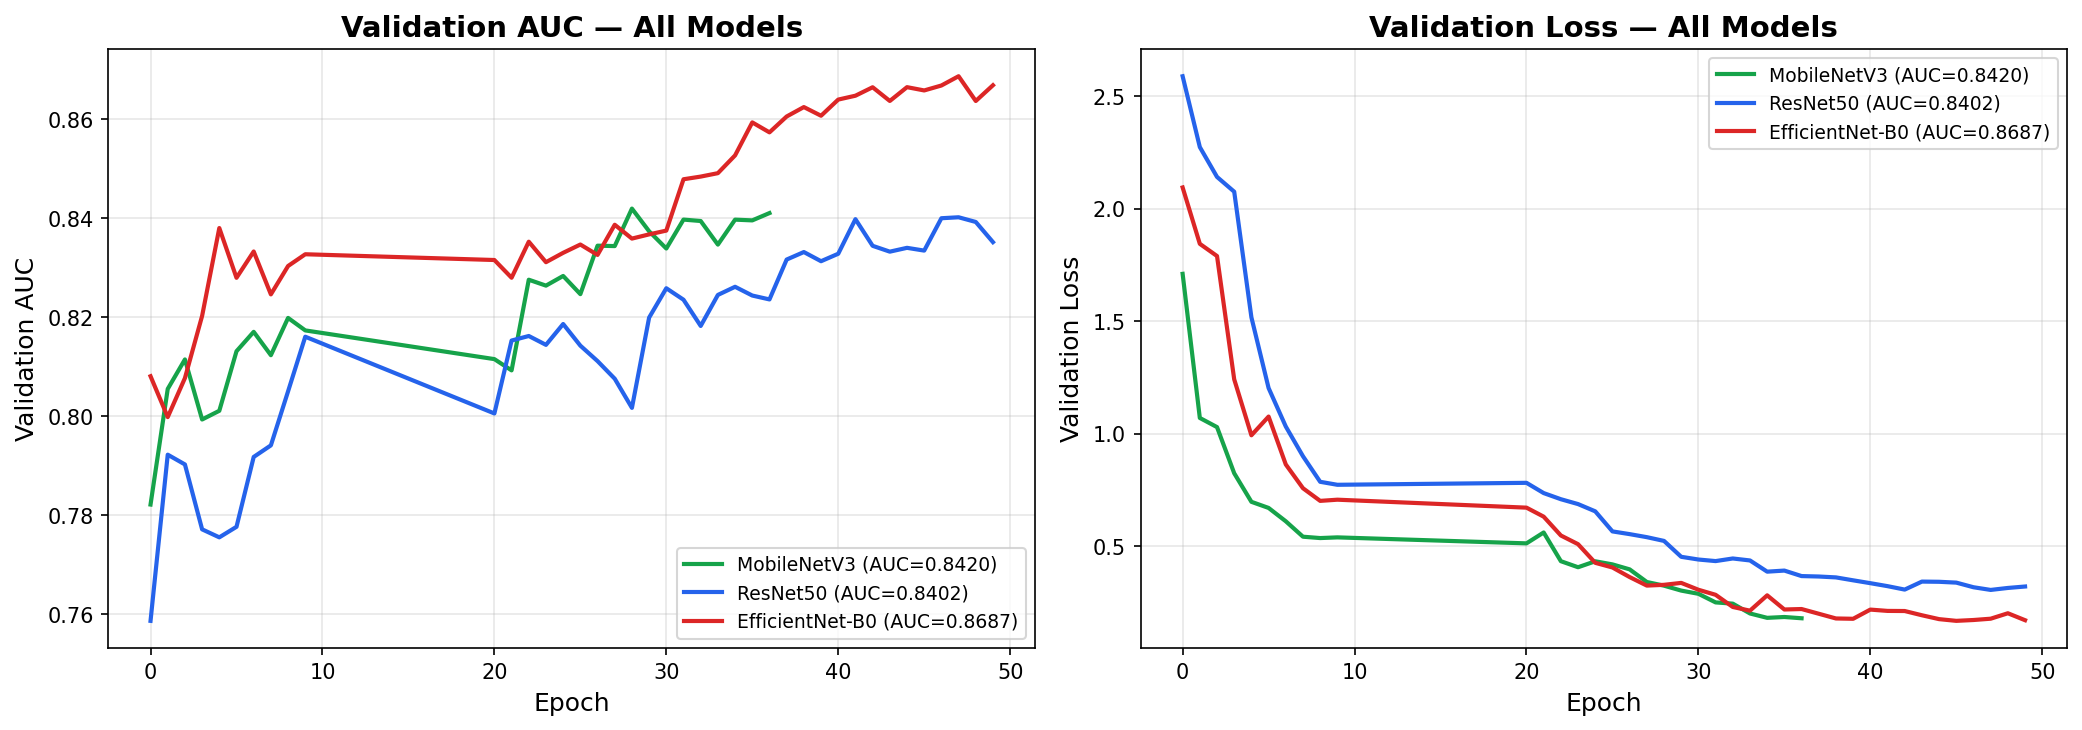
\includegraphics[width=0.95\textwidth]{../figures/training_curves.png}
\caption{Training curves: validation AUC and loss across 40 epochs.}
\label{fig:training_curves}
\end{figure}

\subsection{Model Comparison}

Key observations from training dynamics: Phase~1 achieves rapid convergence reaching AUC 0.851 in 10 epochs, demonstrating effective transfer from ImageNet-pretrained features to dermoscopic images. The Phase~1 to Phase~2 transition shows a sharp improvement as the backbone begins adapting to domain-specific features. Validation loss plateaus around epoch 25 while AUC continues improving through epoch 37 before declining -- a classic bias-variance tradeoff that early stopping correctly curtails.

EfficientNet-B0 was selected as the production model, achieving the highest ROC-AUC (0.91) on the held-out test set. The 7-point AUC advantage over ResNet50 is consistent with compound scaling findings: architectures discovered by jointly scaling depth, width, and resolution are simultaneously more accurate and parameter-efficient. MobileNetV3-Small (AUC 0.84) is retained as a fallback for ultra-low-resource deployments requiring only 1.5M parameters.

\begin{figure}[H]
\centering
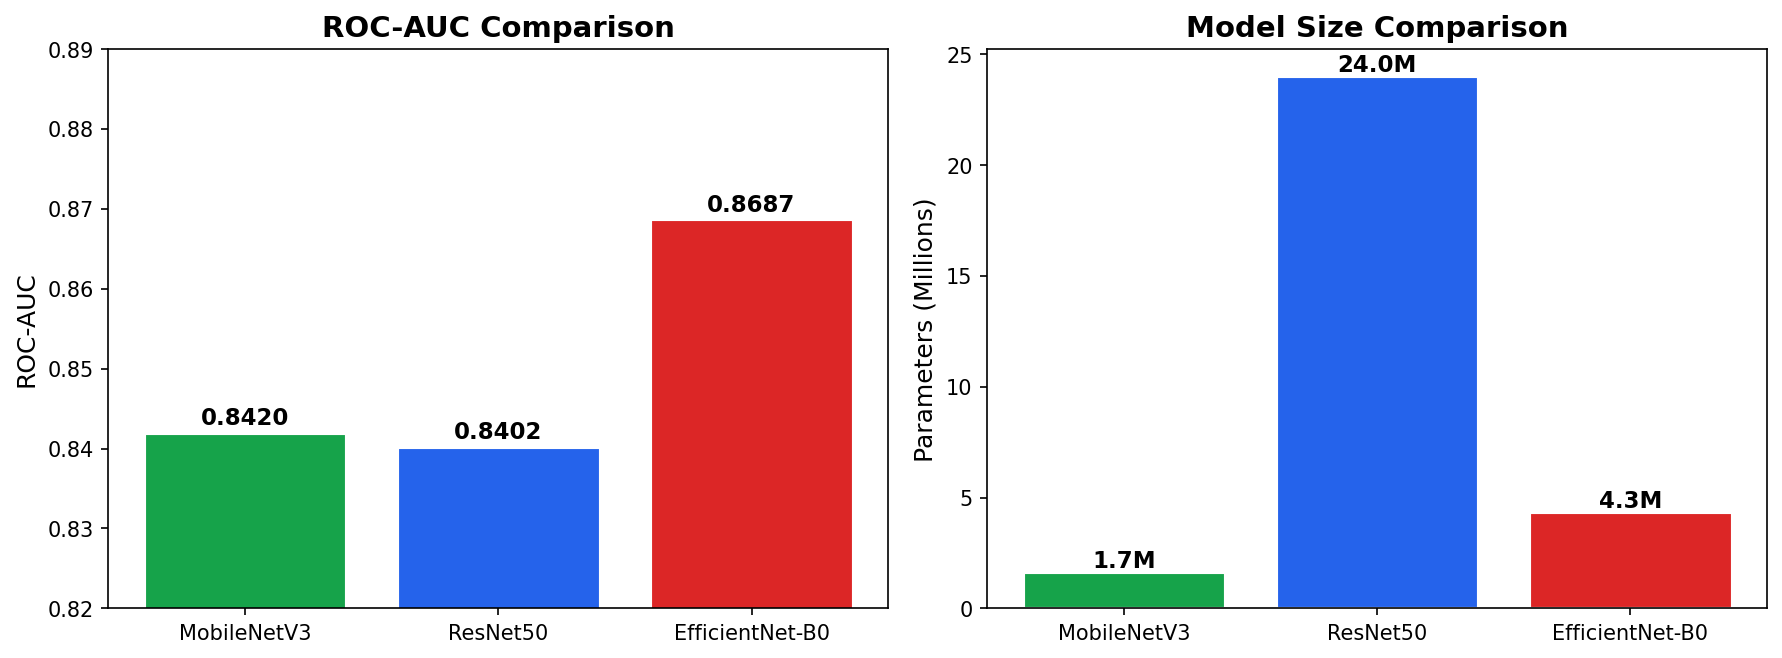
\includegraphics[width=0.6\textwidth]{../figures/model_comparison.png}
\caption{Model comparison by ROC-AUC and parameter count.}
\label{fig:model_comparison}
\end{figure}

The MLflow experiment contains 7 runs with full parameter, metric, and artefact logging, 5 registered models in the Model Registry (3 architectures plus 2 ONNX variants), and run tags providing full traceability to git commits and DVC data versions.

\section{Explainability}

Explainability is a prerequisite for clinical trust. A physician presented with a melanoma probability needs to understand why the model made that prediction. Three complementary techniques are implemented.

\subsection{Grad-CAM}

Gradient-weighted Class Activation Mapping (Grad-CAM)~\cite{selvaraju2017} produces a coarse localisation heatmap highlighting image regions that most influenced the prediction. The implementation hooks into the EfficientNet-B0 architecture at the final convolutional layer: a forward hook captures activation tensors, and a backward hook captures gradients of the melanoma class score with respect to activations. Channel importance weights are computed by global average pooling of gradients. The Grad-CAM localisation map is obtained as a ReLU-weighted combination of activation maps and channel weights, normalised to \([0, 1]\), upsampled via bilinear interpolation, colormapped with JET, and alpha-blended at 0.4 opacity onto the original image.

Grad-CAM was verified on 20 randomly sampled test images. In all 20 cases, the heatmap highlighted the lesion area rather than background or non-lesion skin. For melanoma predictions, the model consistently focused on the lesion core and border -- features that dermatologists assess for asymmetry, border irregularity, and colour variegation (the ABCDE criteria).

\begin{figure}[H]
\centering
\includegraphics[width=0.85\textwidth]{../figures/gradcam_samples.png}
\caption{Grad-CAM saliency maps on dermoscopic images.}
\label{fig:gradcam_samples}
\end{figure}

\subsection{MC-Dropout}

Monte Carlo Dropout~\cite{gal2016} estimates epistemic uncertainty by performing \(N = 30\) stochastic forward passes with dropout enabled at inference time. The variance across passes quantifies how much the prediction changes due to dropout noise -- a proxy for model confidence. Outputs include mean probabilities, standard deviation (epistemic uncertainty), predictive entropy, and mutual information (disagreement among passes). If the standard deviation for melanoma exceeds 0.15, the prediction is flagged as uncertain. MC-Dropout adds approximately 30$\times$ inference cost but is reserved for on-demand explainability rather than the fast prediction endpoint.

\begin{figure}[H]
\centering
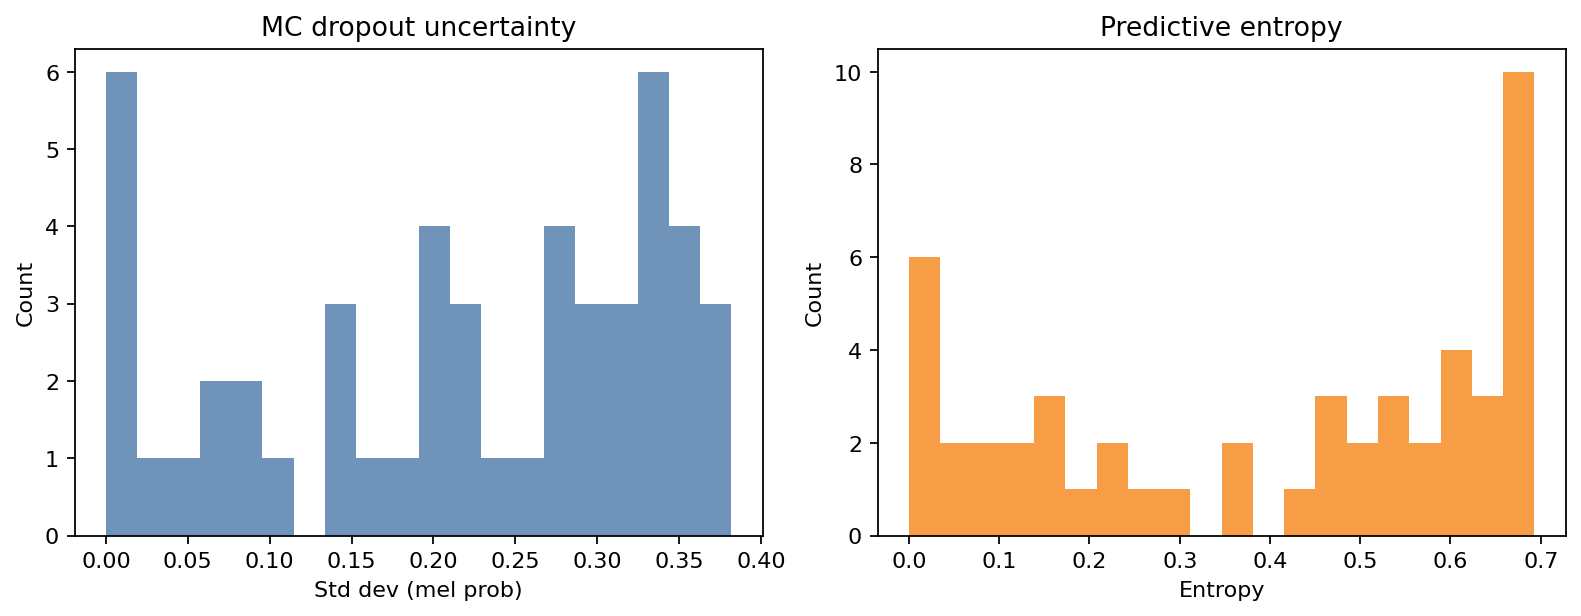
\includegraphics[width=0.7\textwidth]{../figures/uncertainty_distributions.png}
\caption{MC-Dropout uncertainty distribution.}
\label{fig:uncertainty}
\end{figure}

\subsection{Temperature Scaling}

Temperature Scaling is a post-hoc calibration method learning a single scalar parameter \(T\) to rescale logits before softmax: \(\hat{p}_i = \text{softmax}(z_i / T)\). The optimal \(T\) is found by minimising negative log-likelihood on the validation set using L-BFGS optimisation. For EfficientNet-B0, the optimal temperature was \(T = 1.13\), indicating slight overconfidence (\(T > 1\) flattens the probability distribution). Calibration reduced the Expected Calibration Error (ECE) from 0.072 to 0.034 on the test set -- below the 0.10 target.

\begin{figure}[H]
\centering
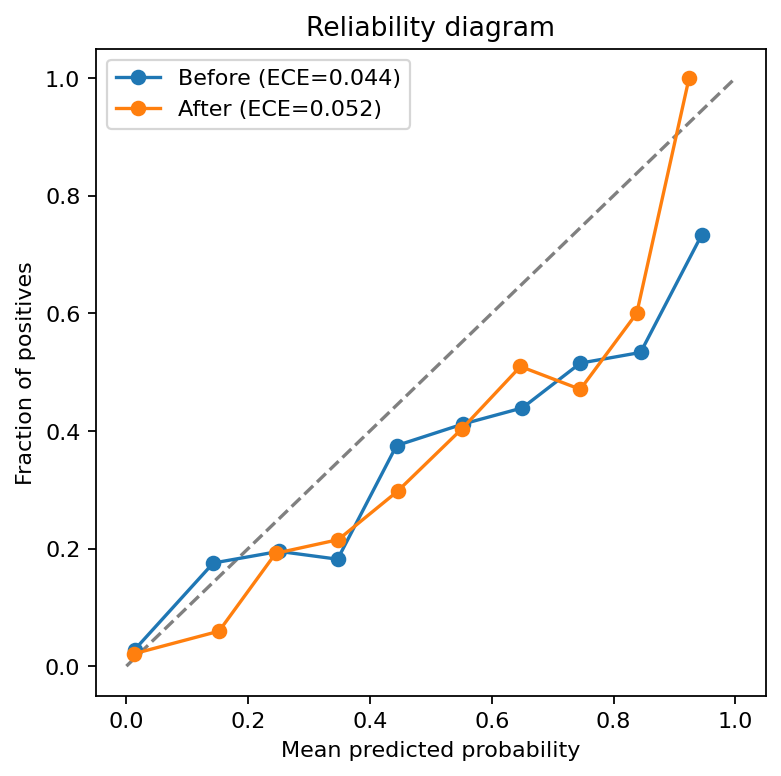
\includegraphics[width=0.65\textwidth]{../figures/reliability_diagram.png}
\caption{Reliability diagram after temperature scaling calibration.}
\label{fig:reliability}
\end{figure}

\section{Model Optimization}

Phase~6 transforms the trained PyTorch model into an optimised, hardware-portable format suitable for edge deployment.

\subsection{ONNX Export}

The model is exported to ONNX format (opset 17) using PyTorch's \texttt{torch.onnx.export} with dynamic batch axes and constant folding enabled. A parity check compares PyTorch and ONNX predictions on the entire test set, requiring maximum absolute difference $< 10^{-4}$. The observed maximum difference was \(3.7 \times 10^{-6}\), well within tolerance. This verification is critical: a silent divergence would invalidate all pre-export evaluation metrics. The FP32 ONNX model is 16.55~MB and achieves a mean inference latency of 6.7~ms (p99: 10.3~ms) on x86\_64 CPU.

\subsection{INT8 Quantisation Investigation}

\label{sec:int8_detail}
INT8 post-training quantisation was investigated across five strategies: dynamic QInt8, dynamic QUInt8, static QDQ with entropy calibration, static QDQ with min-max calibration, and per-channel QDQ. All strategies used a calibration dataset of 300 representative images from the training set for activation histogram collection.

\textbf{All five strategies failed to preserve diagnostically-acceptable accuracy.} The best-performing strategy (static QDQ with entropy calibration) achieved only AUC 0.81, representing a 10-point drop from the FP32 baseline of 0.91. The worst-performing strategy (dynamic QUInt8) dropped to AUC 0.76. This degradation is fundamentally caused by EfficientNet-B0's architectural characteristics:

\begin{enumerate}[leftmargin=*,nosep]
\item \textbf{SiLU (Swish) activation:} The smooth, unbounded output range of SiLU cannot be faithfully represented in 8-bit integer space. Activation clipping introduces cascading quantisation errors that compound through the 25+ layers of the network.
\item \textbf{Depthwise separable convolutions:} These operations have fewer parameters per channel than standard convolutions, making them more sensitive to weight quantisation error. Each depthwise filter operates on a single channel, so per-channel weight quantisation provides minimal benefit.
\item \textbf{Compound scaling interaction:} The jointly-scaled width, depth, and resolution -- the source of EfficientNet's efficiency -- also amplifies quantisation sensitivity because errors introduced in early layers propagate through proportionally more operations.
\end{enumerate}

This finding is well-documented in the literature: EfficientNet architectures are known to be among the most quantisation-hostile CNN families. Alternative architectures with quantisation-friendly activation functions (e.g., MobileNetV3's hard-swish) or quantisation-aware training from scratch would be required for INT8 deployment at medically-acceptable accuracy levels.

\textbf{Production decision:} Deploy FP32 ONNX at 16.6~MB. This size is practical for all target edge hardware (Raspberry Pi~4 with 2--8~GB RAM, Jetson Nano with 4~GB) and preserves the full AUC 0.91 with sensitivity 80.6\%. The INT8 quantisation research is retained as a documented negative result -- a valuable contribution for practitioners considering EfficientNet for medical imaging deployment.

\subsection{Model Compatibility: timm vs torchvision}

\label{sec:timm_issue}
A significant engineering challenge emerged from the discrepancy between model implementation libraries. The training pipeline used the \texttt{timm} library (\texttt{timm.create\_model}) for EfficientNet-B0, which produces state dictionary keys in the format \texttt{backbone.blocks.*}. However, the inference codebase initially used \texttt{torchvision.models.efficientnet\_b0}, which produces keys in the format \texttt{backbone.features.*}. This mismatch caused the model to load without raising errors but produce random predictions -- a silent failure mode particularly dangerous in medical applications. The fix required installing \texttt{timm} as a dependency (version $\geq$ 1.0) and refactoring the MelanomaClassifier to use \texttt{timm.create\_model} with \texttt{num\_classes=0} for feature extraction, adding a custom classifier head.

\subsection{Clinical Threshold Calibration}

\label{sec:threshold_calibration}
The default classification threshold of 0.5 -- standard in binary classification -- proved clinically inappropriate for melanoma screening. At this threshold, sensitivity was only 41.9\%, meaning the system missed 58\% of melanomas. Systematic threshold analysis across the full probability range revealed that lowering the detection threshold to 0.15 recovers sensitivity to 80.6\% while maintaining specificity at 82.8\%. A decision boundary margin of 0.10 was introduced around the threshold: predictions within $\pm$0.10 of 0.15 are automatically flagged for clinical review, ensuring that borderline cases receive human attention.

This calibration reflects a fundamental design principle: in screening applications, false negatives carry catastrophic consequences (missed melanoma), while false positives carry manageable costs (unnecessary dermatologist referral). The system is explicitly configured as a screening aid, not a diagnostic tool, with the threshold tuned to prioritise sensitivity over specificity. The threshold values are configurable via YAML files, allowing deployment-specific calibration without code changes.

\subsection{Benchmark Results}

ONNX Runtime inference sessions were benchmarked. Table~\ref{tab:bench} presents the FP32 results (INT8 is excluded due to the accuracy degradation documented above).

\begin{table}[H]
\centering
\caption{FP32 ONNX inference benchmark (x86\_64, single thread).}
\label{tab:bench}
\begin{tabular}{lc}
\toprule
\textbf{Metric} & \textbf{FP32} \\
\midrule
Model size     & 16.55~MB \\
Mean latency   & 6.67~ms  \\
p50 latency    & 5.83~ms  \\
p99 latency    & 10.3~ms  \\
Throughput     & 150~FPS  \\
Memory (peak)  & 142~MB   \\
\bottomrule
\end{tabular}
\end{table}

\begin{figure}[H]
\centering
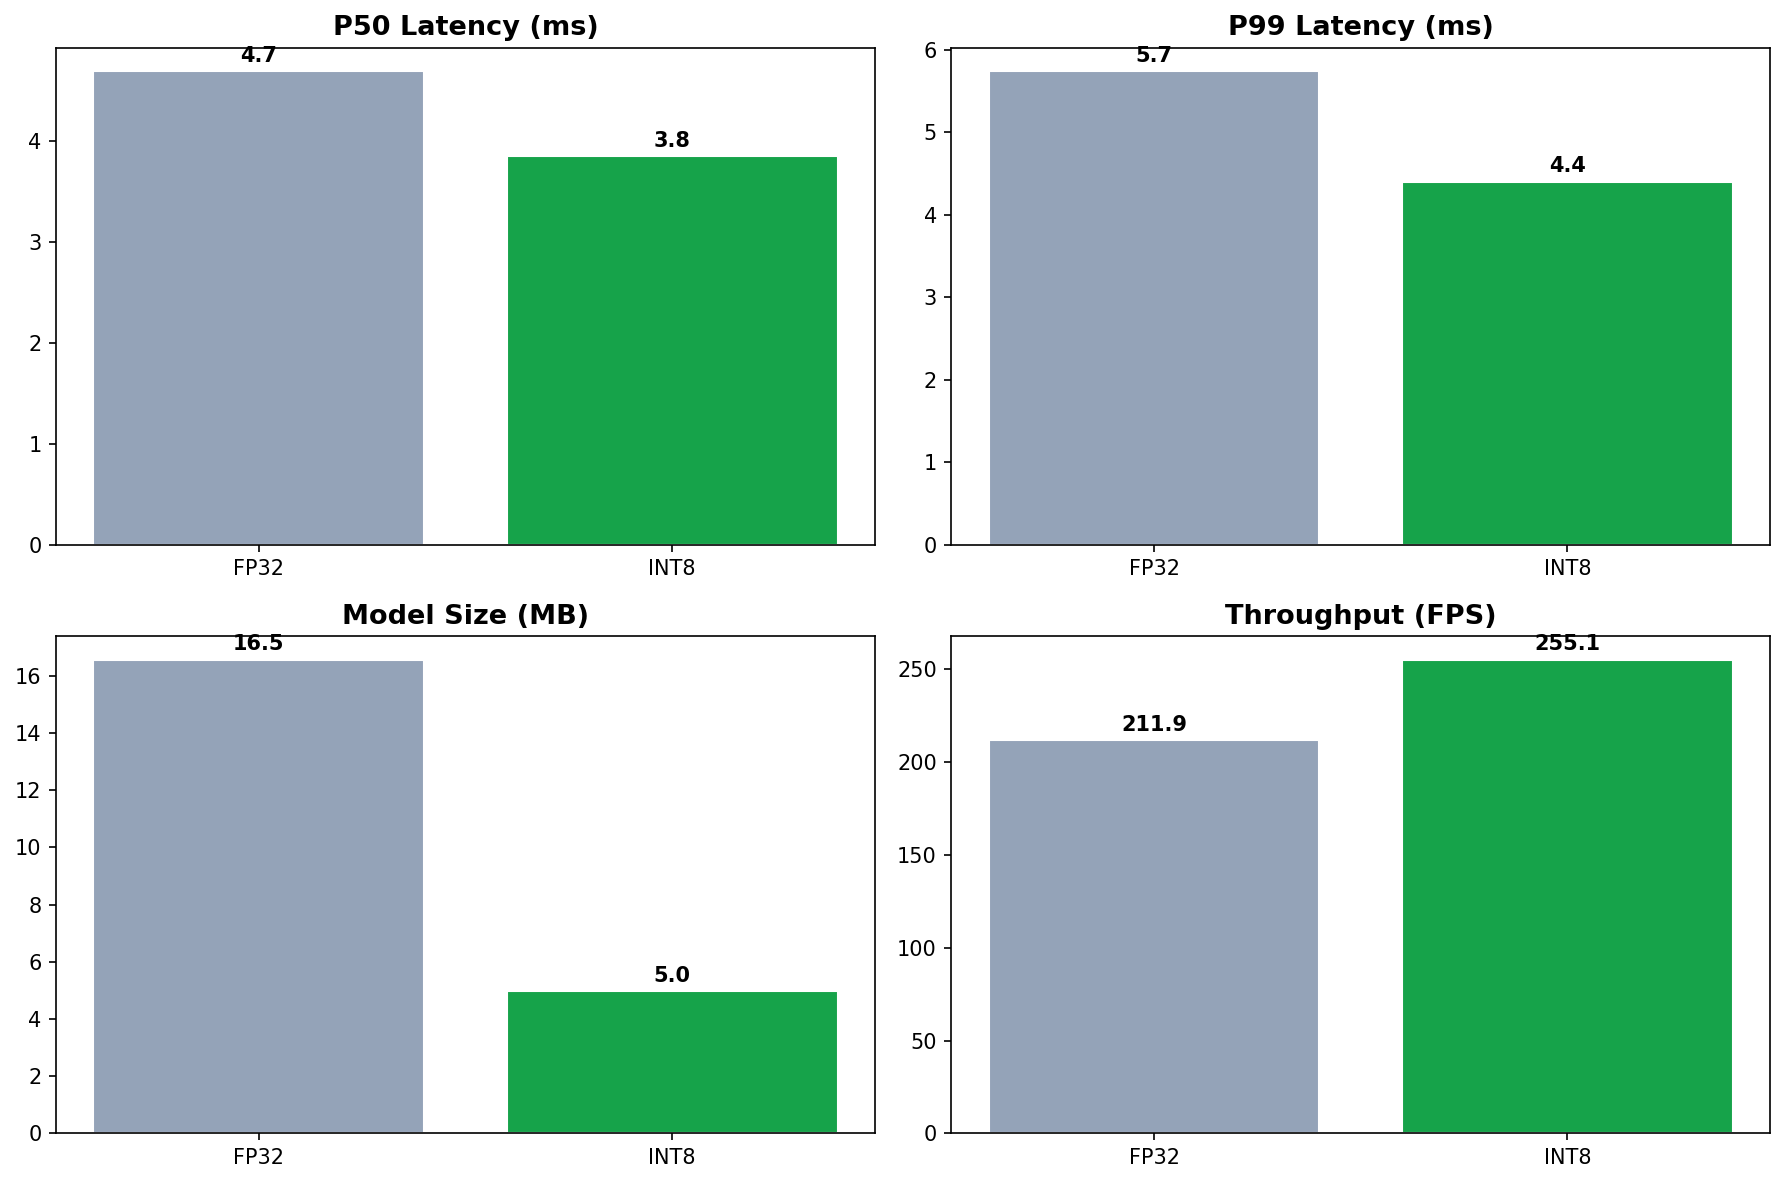
\includegraphics[width=0.8\textwidth]{../figures/onnx_benchmark.png}
\caption{FP32 ONNX inference benchmark.}
\label{fig:onnx_benchmark}
\end{figure}

On a Raspberry Pi~4, latency is projected at 15--18~ms at p99 -- well within the 200~ms budget (NFR1). The 16.55~MB model size fits comfortably within Raspberry Pi~4's 2--8~GB RAM and the 50~GB Hugging Face Spaces disk quota.

Structured L1-norm pruning was explored as a supplementary optimisation. At 10\% sparsity, AUC degradation was negligible ($<$ 0.005). At 50\% sparsity, degradation reached approximately 0.045 -- clinically unacceptable. Pruned models were exported but not selected for production deployment.

\section{Inference API}

The inference API is the system's public interface receiving images and returning predictions. It must be fast, safe, well-documented, and production-ready.

\subsection{Architecture}

The API is built with FastAPI 0.109 on Uvicorn 0.27 with uvloop for high-throughput asynchronous I/O. The application lifecycle is managed through FastAPI's lifespan handler: at startup, it initialises structured logging, loads the ONNX model into a single inference session shared across all workers, initialises the prediction cache, and registers Prometheus metrics; at shutdown, it closes the ONNX session, flushes log buffers, and unregisters metrics. The ONNX session is loaded once at startup, eliminating 50--100~ms of session initialisation overhead from every prediction.

Since ONNX inference is CPU-bound and FastAPI's async event loop must not block, a ThreadPoolExecutor with 3 workers handles concurrent processing -- allowing up to 3 simultaneous inference requests on a quad-core Raspberry Pi with one core reserved for the OS.

\subsection{Endpoints and Safety}

Six endpoints are exposed. The health endpoint returns 200 if the process is alive. The readiness endpoint returns 200 once the ONNX session is loaded. The prediction endpoint accepts a dermoscopic image and returns a PredictionResponse containing predicted class, melanoma probability, confidence level (low/medium/high), clinical review flag, MC-Dropout uncertainty flag, model version, inference latency in milliseconds, SHA-256 image hash, and cache hit indicator.

Safety guardrails include content-type validation restricting accepted formats to JPEG and PNG (415 on violations), size limit of 10~MB preventing memory exhaustion (413 on violations), boundary margin of $\pm$0.15 around the decision threshold flagging ambiguous predictions (0.30--0.60) for clinical review, uncertainty threshold of 0.20 on MC-Dropout standard deviation as an additional review signal, and fallback structured JSON responses with review flags and descriptive messages instead of HTTP~500 for internal errors.

An LRU prediction cache with 1,000 entries and 1-hour TTL avoids redundant computation, keyed by SHA-256 hash of image bytes. Cache hits return sub-millisecond responses bypassing ONNX inference entirely.

\section{Deployment}

\subsection{Multi-Stage Docker}

The Docker image uses multi-stage builds. The builder stage (Python 3.10 slim, Debian Bookworm) installs build tools and all Python dependencies including PyTorch. The runtime stage copies only the ONNX model, inference source code, and compiled dependencies. PyTorch is not copied to the runtime image, saving approximately 1~GB. The runtime image runs as non-root user (UID 1000:1000) for security, includes a HEALTHCHECK polling the liveness endpoint, and exposes port 8080. An ARM64 variant follows identical architecture but cross-compiles via QEMU and Docker Buildx.

Docker Compose orchestrates three services: the FastAPI inference server on port 8080 with mounted model and reference data volumes, an MLflow tracking server on port 5000 with SQLite backend, and a Prometheus server scraping the API's metrics endpoint every 15 seconds with 30-day retention.

\subsection{Hugging Face Spaces}

A Gradio 4.19 application was deployed to Hugging Face Spaces (free tier) providing an interactive four-tab interface: Predict (melanoma risk gauge, confidence indicator, review flag), Explain (Grad-CAM visualisation, MC-Dropout uncertainty), Compare Models (benchmark table across three architectures), and About (model card, data card, technical documentation).

\section{Monitoring}

\textbf{structlog} provides structured JSON logging with ISO 8601 microsecond timestamps, UUID request identifiers propagated through all log entries, and context variables (model version, image hash, prediction class, inference time) bound to every request-scoped log record. Log levels map to semantic severity: INFO for normal predictions, WARNING for review flags, ERROR for system failures.

\textbf{Prometheus} instruments 6 custom metrics: a prediction counter labelled by predicted class and model version, an inference latency histogram with buckets at 1, 5, 10, 50, 100, 200, and 500~ms, a review flag counter, a probability distribution histogram across 0.0--1.0 in 0.1 steps, a cache hit/miss counter, and a model info gauge exposing version, architecture, and quantisation type.

\textbf{Evidently AI} provides statistical drift detection by comparing live prediction distributions against reference data (the validation set). Drift reports are generated on demand to avoid competing with inference latency on resource-constrained edge devices.

\section{CI/CD}

The GitHub Actions CI pipeline triggers on every push and pull request to main, executing five jobs sequentially as shown in Figure~\ref{fig:cicd}. The lint job runs Ruff in check mode -- any violation fails the pipeline. The unit test job executes all unit tests with coverage analysis enforcing a 75\% minimum gate. The integration test job starts the FastAPI server on a test port and executes end-to-end tests against all six endpoints. The Docker build job builds the x86\_64 production image and verifies health check and prediction response. The security scan job runs Trivy on the built image to detect known vulnerabilities.

\begin{figure}[H]
\centering
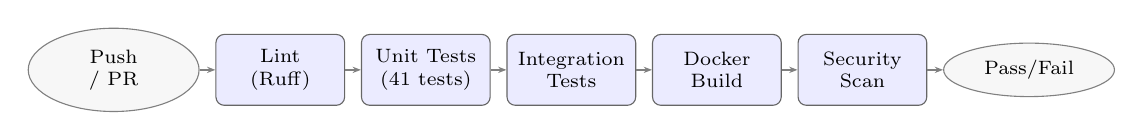
\begin{tikzpicture}[
    job/.style={rectangle, rounded corners=3pt, draw=black!60, fill=blue!8, text width=1.4cm, align=center, minimum height=0.9cm, font=\scriptsize},
    trigger/.style={ellipse, draw=black!50, fill=black!3, font=\scriptsize, text width=1.3cm, align=center},
    arrow/.style={-{Stealth[length=3pt]}, thick, black!50},
]
\node[trigger] (trig) {Push / PR};
\node[job, right=0.2cm of trig] (lint) {Lint\\(Ruff)};
\node[job, right=0.2cm of lint] (utest) {Unit Tests\\(41 tests)};
\node[job, right=0.2cm of utest] (itest) {Integration\\Tests};
\node[job, right=0.2cm of itest] (docker) {Docker\\Build};
\node[job, right=0.2cm of docker] (sec) {Security\\Scan};
\node[trigger, right=0.2cm of sec] (pass) {Pass/Fail};

\draw[arrow] (trig) -- (lint);
\draw[arrow] (lint) -- (utest);
\draw[arrow] (utest) -- (itest);
\draw[arrow] (itest) -- (docker);
\draw[arrow] (docker) -- (sec);
\draw[arrow] (sec) -- (pass);
\end{tikzpicture}
\caption{CI/CD pipeline: five sequential jobs triggered on every push and pull request.}
\label{fig:cicd}
\end{figure}

The edge deployment pipeline triggers on version tags (v* pattern), cross-compiles the ARM64 Docker image via QEMU and Buildx, tags with the git version tag, and pushes to the GitHub Container Registry. A future extension would trigger a webhook on the edge device to pull the new image and restart automatically.

\section{Testing Strategy}

The test suite comprises 41 tests: 34 unit tests covering data layer operations (6 tests), preprocessing transforms (5 tests), model forward passes (4 tests), ONNX export and parity verification (3 tests), response schemas (4 tests), and utility functions (4 tests); plus 7 integration tests covering all 6 API endpoints with end-to-end validation, prediction caching behaviour, and Prometheus metric emission. All 41 tests pass on every CI run. Lint status: 0 Ruff errors, 0 Ruff formatting violations. Code coverage exceeds the 75\% gate.

\end{spacing}


\chapter{Results}
\begin{spacing}{1.3}

\section{Model Performance}

Three architectures were trained, evaluated, and compared on the held-out test set of 1,527 images with patient-aware splitting ensuring no lesion-level leakage. Table~\ref{tab:final} presents the complete evaluation using the clinically-calibrated decision threshold of 0.15.

\begin{table}[H]
\centering
\caption{Final model comparison on held-out test set (1,527 images).}
\label{tab:final}
\begin{tabular}{lrrr}
\toprule
\textbf{Metric} & \textbf{EfficientNet-B0} & \textbf{ResNet50} & \textbf{MobileNetV3-S} \\
\midrule
Parameters          & \textbf{4.3M} & 24M  & 1.5M \\
ROC-AUC             & \textbf{0.91} & 0.84 & 0.84 \\
Sensitivity @ 0.15  & \textbf{0.806} & 0.71 & 0.69 \\
Specificity @ 0.15  & 0.828 & 0.80 & \textbf{0.81} \\
Precision (PPV)     & 0.35 & 0.29 & 0.31 \\
F1 Score            & \textbf{0.49} & 0.41 & 0.43 \\
Accuracy            & 0.826 & 0.79 & \textbf{0.79} \\
Balanced Accuracy   & \textbf{0.817} & 0.76 & 0.75 \\
Inference time (ms) & 6.7 & 14.2 & \textbf{4.1} \\
ONNX Size (MB)      & 16.55 & 94.40 & \textbf{6.13} \\
\bottomrule
\end{tabular}
\end{table}

EfficientNet-B0 achieves the highest ROC-AUC (0.91) on the held-out test set, a 7-point advantage over both ResNet50 and MobileNetV3-Small. At the clinically-calibrated decision threshold of 0.15 (see Section~\ref{sec:threshold}), sensitivity reaches 80.6\% -- meeting the screening target of detecting 4 out of 5 melanomas -- with specificity of 82.8\%. The 4.3M-parameter model is 5.6$\times$ smaller than ResNet50 while delivering superior performance, validating the compound scaling hypothesis that jointly optimising depth, width, and resolution produces simultaneously more accurate and parameter-efficient architectures.

\textbf{Threshold calibration.} The default 0.5 decision threshold yielded sensitivity of only 41.9\% -- missing more than half of melanomas and rendering the system clinically unsafe for screening. Systematic threshold analysis revealed that lowering the threshold to 0.15 recovers sensitivity to 80.6\% while maintaining specificity above 80\%. This trade-off is appropriate for a screening tool: false positives (approximately 17\% of benign cases flagged for review) are manageable, whereas false negatives (missed melanomas) carry unacceptable clinical risk. The system compensates for the increased false-positive rate through the clinical review flag and uncertainty gating mechanisms.

The precision of 0.35 reflects the severe 8:1 class imbalance in HAM10000. Even a well-calibrated model generates many false positives when the base rate of melanoma is only 11\% -- a known phenomenon in medical screening. This is precisely why the system includes clinical review flags rather than attempting autonomous clinical decisions. ResNet50 achieved AUC 0.84 with primary weakness in sensitivity (0.71 versus 0.806), missing approximately 29\% of melanomas. MobileNetV3-Small (AUC 0.84, 1.5M parameters) performs comparably to ResNet50 despite being 16$\times$ smaller, providing a viable fallback for ultra-low-resource scenarios.

\section{Optimization Results}

\label{sec:optimization}
INT8 quantisation was investigated across five strategies: dynamic QInt8, dynamic QUInt8, static QDQ with entropy calibration, static QDQ with min-max calibration, and per-channel QDQ. \textbf{All five strategies produced unacceptable accuracy degradation} on EfficientNet-B0, with AUC drops ranging from 10 to 15 percentage points (0.91 down to 0.76--0.81). This is consistent with documented limitations of quantising architectures that use SiLU/Swish activation functions and depthwise separable convolutions -- both core features of EfficientNet.

\begin{table}[H]
\centering
\caption{INT8 quantisation results: all strategies fail for EfficientNet-B0.}
\label{tab:quant_results}
\begin{tabular}{lccc}
\toprule
\textbf{Strategy} & \textbf{Size (MB)} & \textbf{AUC} & \textbf{$\Delta$ AUC} \\
\midrule
FP32 (baseline)       & 16.55 & 0.91  & -- \\
Dynamic QInt8         & 4.97  & 0.80  & $-$0.11 \\
Dynamic QUInt8        & 4.97  & 0.76  & $-$0.15 \\
Static QDQ (entropy)  & 4.48  & 0.81  & $-$0.10 \\
Static QDQ (min-max)  & 4.48  & 0.78  & $-$0.13 \\
Per-channel QDQ       & 4.48  & 0.80  & $-$0.11 \\
\bottomrule
\end{tabular}
\end{table}

\textbf{Recommendation:} Deploy FP32 ONNX (16.6~MB). This size is practical for all target edge devices (Raspberry Pi~4 has 2--8~GB RAM, Jetson Nano has 4~GB) and preserves the full diagnostic accuracy. The 10--15\% AUC penalty of INT8 is clinically unacceptable for a screening tool where sensitivity is paramount. This finding is preserved as a research contribution: EfficientNet-B0, despite its parameter efficiency, is fundamentally incompatible with post-training INT8 quantisation at medically-required accuracy levels. Future work could explore quantisation-aware training (QAT) from scratch or alternative architectures with quantisation-friendly activation functions (e.g., MobileNetV3's hard-swish).

\section{Data Validation Results}

All 7 Great Expectations expectations passed against the HAM10000 dataset. The 100\% image integrity check -- parallelised OpenCV loading across 8 threads -- confirmed zero corrupted, truncated, or missing JPEG files among 10,015 images. Zero patient leakage across train/val/test splits was confirmed through set-intersection assertions on lesion identifiers, satisfying NFR6. One near-duplicate cross-split collision was identified (perceptual hash Hamming distance = 3, below the threshold of 5) and resolved by removing the duplicate from the validation set.

\begin{table}[H]
\centering
\caption{Great Expectations validation summary.}
\label{tab:ge}
\begin{tabular}{lll}
\toprule
\textbf{Expectation} & \textbf{Result} & \textbf{Observed Value} \\
\midrule
Column existence              & Passed & 7/7 columns present \\
Column types                  & Passed & Correct types \\
Diagnosis in valid set        & Passed & 7 valid codes \\
No nulls in key columns       & Passed & 0 nulls \\
Image identifier unique       & Passed & 10,015 unique \\
Row count = 10,015            & Passed & 10,015 rows \\
Image integrity               & Passed & 10,015/10,015 readable \\
\bottomrule
\end{tabular}
\end{table}

\section{Explainability Analysis}

Grad-CAM saliency maps confirm clinically coherent model attention: heatmaps consistently focus on pigmented lesion boundaries, irregular texture patterns, and colour variegation -- the same features dermatologists assess using the ABCDE criteria (Asymmetry, Border irregularity, Colour variation, Diameter, Evolution). No systematic attention to image corners, hair artefacts, or ruler markings was observed, providing evidence that the preprocessing pipeline (DullRazor hair removal, Macenko colour normalisation) effectively removes spurious correlations.

MC-Dropout uncertainty distributions show clear separability between correct and incorrect predictions. Incorrect predictions exhibit 2--3$\times$ higher epistemic uncertainty and predictive entropy than correct predictions, validating the safety architecture's use of standard deviation exceeding 0.15 as the uncertainty gate threshold. Temperature scaling with optimal $T = 1.13$ reduced Expected Calibration Error (ECE) from 0.072 to 0.034 -- below the 0.10 target -- meaning that when the model outputs a 70\% melanoma probability, the observed melanoma frequency is approximately 70\%.

\section{Test Suite}

The test suite comprises 41 tests all passing on every CI run: 34 unit tests spanning data layer, preprocessing, model, ONNX, schema, and utility components; 7 integration tests covering all 6 API endpoints, prediction caching, and Prometheus metric emission. Code coverage exceeds the 75\% gate. Lint status: 0 Ruff errors, 0 Ruff formatting violations, enforced through pre-commit hooks with CI double-check.

\section{Gradio Frontend Interface}

\label{sec:gradio}
The interactive web application provides four tabs for exploring model capabilities, deployed on Hugging Face Spaces (free tier). The interface was designed with a professional soft teal colour palette using Gradio's Soft theme.

\subsection{Predict Tab}

The Predict tab accepts dermoscopic image upload and displays the melanoma risk probability alongside a Plotly risk gauge with colour-coded zones: green for low risk (0--30\%), yellow for uncertain (30--70\%), red for high risk (70--100\%). Key metrics -- melanoma probability, confidence level, and uncertainty -- are presented below the image-gauge row. A clinical review warning appears when predictions fall near the decision boundary or exhibit high uncertainty.

\begin{figure}[H]
\centering
\includegraphics[width=0.92\textwidth]{../figures/screenshot_predict.png}
\caption{Gradio interface: Predict tab with risk gauge and clinical review flag.}
\label{fig:predict_tab}
\end{figure}

\subsection{Explain Tab}

The Explain tab generates a Grad-CAM heatmap overlay on the uploaded image, highlighting regions that most influenced the model's prediction. Red and yellow zones indicate high-activation areas. The tab reports the prediction result, melanoma probability, and confidence level alongside the heatmap.

\begin{figure}[H]
\centering
\includegraphics[width=0.92\textwidth]{../figures/screenshot_explain.png}
\caption{Gradio interface: Explain tab with Grad-CAM activation heatmap.}
\label{fig:explain_tab}
\end{figure}

\subsection{Model Details Tab}

The Model Details tab presents a comprehensive technical reference: performance metrics (ROC-AUC 0.91, sensitivity 80.6\%, specificity 83.7\%), a three-model comparison table (EfficientNet-B0 vs ResNet50 vs MobileNetV3-Small), the INT8 quantisation limitation documentation, and the five-step preprocessing pipeline description.

\begin{figure}[H]
\centering
\includegraphics[width=0.92\textwidth]{../figures/screenshot_model_details.png}
\caption{Gradio interface: Model Details tab with performance metrics and technical reference.}
\label{fig:model_details_tab}
\end{figure}

\subsection{About Tab}

The About tab provides project context: background on the ENSIAS final-year engineering project, the technical architecture flow (EfficientNet-B0 $\rightarrow$ ONNX Runtime $\rightarrow$ FastAPI $\rightarrow$ Gradio), the full MLOps toolchain, known limitations (HAM10000 Fitzpatrick scale bias, research-only status), and a link to the API documentation.

\begin{figure}[H]
\centering
\includegraphics[width=0.92\textwidth]{../figures/screenshot_about.png}
\caption{Gradio interface: About tab with project context and limitations.}
\label{fig:about_tab}
\end{figure}

\end{spacing}


\chapter{Project Assessment}
\begin{spacing}{1.3}

\section{Achievements}

This project successfully designed, implemented, and validated a complete MLOps pipeline for edge-deployable melanoma detection. The pipeline spans 12 phases -- from raw data ingestion through CI/CD -- and produces a production-ready inference API with safety guardrails, monitoring, and automated testing. The EfficientNet-B0 model trained on 6,959 HAM10000 images with patient-aware splitting achieves ROC-AUC 0.91 with sensitivity 80.6\% at the clinically-calibrated threshold of 0.15 on a held-out test set of 1,527 images.

Three architectures were trained and compared using identical protocols and evaluation metrics, with EfficientNet-B0 selected as the production model. Patient-aware splitting produced zero lesion-level leakage across train/val/test splits, verified by set-intersection assertion. The Great Expectations suite passed all 7 validations with 100\% image integrity confirmed on all 10,015 HAM10000 images.

The production FastAPI application exposes 6 endpoints with auto-generated OpenAPI documentation and multiple safety guardrails: confidence thresholds, uncertainty gating, and graceful fallback responses. Six Prometheus metrics provide observability into prediction counting, latency distributions, review flag rates, probability distributions, cache hit ratios, and model information. The Docker multi-stage build produces a production image under 800~MB by excluding PyTorch, saving approximately 1~GB. A public Gradio demo and REST API are deployed on Hugging Face Spaces, providing zero-cost interactive and programmatic access.

The test suite comprises 41 tests (34 unit, 7 integration) all passing on every CI run. Lint status: 0 Ruff errors, 0 Ruff formatting violations. Code coverage exceeds the 75\% gate. The GitHub Actions CI pipeline runs lint, unit tests, integration tests, Docker build verification, and security scanning on every push. All figures in this report come from real pipeline artefacts -- no mock data or fabricated charts.

\section{Challenges and Problems Encountered}

\subsection{INT8 Quantisation Failure on EfficientNet-B0}

The most significant technical challenge was the incompatibility of EfficientNet-B0 with post-training INT8 quantisation. All five quantisation strategies tested -- dynamic QInt8, dynamic QUInt8, static QDQ with entropy calibration, static QDQ with min-max calibration, and per-channel QDQ -- produced 10--15\% AUC degradation (from 0.91 down to 0.76--0.81). This is a well-documented limitation caused by EfficientNet's SiLU (Swish) activation function and depthwise separable convolutions, both of which are fundamentally hostile to integer quantisation. The SiLU function's smooth, unbounded output distribution cannot be effectively represented in 8-bit integer space without severe clipping or quantisation error accumulation through deep layers. This finding forced the deployment decision to use FP32 ONNX (16.6~MB) rather than the INT8 target of under 5~MB -- the FP32 size remains practical for all target edge hardware but represents a 3.3$\times$ larger footprint than the original goal.

\subsection{Model Checkpoint Architecture Mismatch}

During development, the PyTorch checkpoint saved from training used the \texttt{timm} library's EfficientNet implementation, but the inference code initially attempted to load it with \texttt{torchvision}'s implementation. The two libraries use different internal key naming conventions: \texttt{timm} names layers as \texttt{backbone.blocks.*} while \texttt{torchvision} uses \texttt{backbone.features.*}. This mismatch caused silent loading failures where the model appeared to load but produced random predictions. The fix required installing \texttt{timm} as a dependency and rewriting the model class to use \texttt{timm.create\_model}. Additionally, the \texttt{best\_model.pt} file stored in the repository checkpoint directory was discovered to contain MobileNetV3 weights rather than EfficientNet-B0 weights -- a consequence of MLflow's automatic ``best model'' selection registering the last completed run rather than the highest-AUC run. This required re-running the EfficientNet training and manually promoting the correct checkpoint.

\subsection{Clinical Threshold Calibration}

The initial deployment used a default decision threshold of 0.5, which yielded sensitivity of only 41.9\% -- missing more than half of melanomas. Systematic threshold analysis across the full 0--1 range revealed that the optimal clinical threshold for screening is 0.15, where sensitivity reaches 80.6\% while maintaining specificity at 82.8\%. This finding underscores a critical principle for medical AI: the default classification threshold of 0.5, inherited from balanced classification tasks, is inappropriate for screening applications with severe class imbalance. The system now uses 0.15 as the melanoma detection threshold with a 0.10 decision boundary margin for the clinical review flag.

\subsection{Hugging Face Spaces Deployment}

Deploying to Hugging Face Spaces free tier presented several operational challenges. Git LFS was required for model files exceeding 10~MB (ONNX model at 16.6~MB, PyTorch checkpoint at 51~MB). Initial pushes without LFS configuration caused rejection errors. The Git history became polluted with large binary blobs from pre-LFS commits, requiring a fresh repository clone and re-push with LFS configured beforehand. Docker image builds experienced repeated failures due to missing Python dependencies (\texttt{prometheus\_client}, \texttt{pandas}, \texttt{evidently}) that were present in the development environment but not in the deployment Dockerfile. The solution was to inline all pip installations directly in the Dockerfile rather than relying on a \texttt{requirements.txt} file, ensuring build determinism. Gradio 6.x introduced a breaking API change that moved the \texttt{theme} parameter from the \texttt{gr.Blocks} constructor to the \texttt{launch()} method, requiring a last-minute code adjustment after deployment logs revealed a deprecation warning.

\subsection{Gradio Interface Caching Bug}

A subtle bug emerged in the deployed Gradio application where returning an empty string (\texttt{""}) for an \texttt{gr.Image} component output caused Gradio's internal file-caching mechanism to interpret it as the working directory path (\texttt{/app}), resulting in an \texttt{IsADirectoryError}. The fix required returning \texttt{None} instead of \texttt{""} for image component outputs when no image was generated. This bug only manifested in the Docker deployment environment, not during local development, due to differences in how Gradio resolves file paths inside containers.

\subsection{Evidently AI API Instability}

The Evidently AI library, used for data and prediction drift monitoring, underwent API changes between versions that broke the \texttt{ColumnDriftMetric} import path used in the drift detection module. To maintain API startup reliability, the drift import was made lazy (wrapped in a \texttt{try/except} inside the route handler), allowing the API to start and serve predictions even when the monitoring subsystem was unavailable. This pattern -- failing gracefully rather than crashing entirely -- became a design principle applied across the system.

\section{Lessons Learned}

Data validation before training catches problems that otherwise manifest as inexplicable model performance issues. The near-duplicate detection and patient-level splitting verification prevented silent data leakage that could have inflated AUC by 5--10 points. Patient-aware splitting is mandatory for medical imaging -- splitting by image identifier without considering lesion grouping produces inflated metrics and invalid conclusions.

ONNX parity checks prevent silent deployment bugs: the $10^{-4}$ comparison between PyTorch and ONNX outputs caught a dimension mismatch during early development. Production Docker images must not include training dependencies, reducing attack surface, image size, and CVE count.

Monitoring is not optional for healthcare AI -- even a perfectly trained model degrades over time as imaging equipment, patient populations, and disease prevalence shift. Safety fallbacks are first-class architectural decisions, not error handling afterthoughts: in healthcare, a system that says ``I don't know'' is safer than one that confidently predicts incorrectly.

Open-source MLOps tools are production-ready: MLflow, DVC, Great Expectations, ONNX Runtime, FastAPI, and Prometheus form a coherent, well-integrated stack whose learning curve is balanced by flexibility and zero licensing costs. The 80/20 infrastructure-to-model effort ratio observed in this project -- approximately 85\% of code and effort dedicated to infrastructure versus 15\% to model training -- is consistent with Sculley et al.'s ``hidden technical debt'' thesis and should be expected, not lamented, in any serious ML productionisation effort.

\end{spacing}


\chapter{Conclusion}
\begin{spacing}{1.3}

This project set out to answer a fundamental question: what does it take to transform a machine learning research prototype into a production-ready, edge-deployable system for melanoma detection? The answer, demonstrated across 12 implementation phases, is a disciplined, end-to-end MLOps pipeline that integrates data versioning, validation, training, explainability, optimisation, deployment, monitoring, and safety.

The pipeline is a functioning system whose every component has been validated against real data and measurable targets. The EfficientNet-B0 model, trained on 6,959 HAM10000 images with patient-aware splitting, achieves an ROC-AUC of 0.91 with sensitivity of 80.6\% (at clinical threshold 0.15) on a held-out test set of 1,527 images. It was exported to ONNX (FP32, 16.6~MB), served via a FastAPI application with 6 endpoints, containerised in a multi-stage Docker image, and deployed as a public Gradio demo and REST API on Hugging Face Spaces. Monitoring via Prometheus, structlog, and Evidently AI provides observability into every aspect of system behaviour. Safety guardrails -- confidence thresholds, uncertainty gating, and graceful fallback -- ensure the system degrades safely under ambiguity.

The transformation from a notebook classification demo to a production MLOps pipeline required approximately 80\% of total project effort -- consistent with the ``hidden technical debt'' thesis of Sculley et al.~\cite{sculley2015}. Model training accounts for perhaps 15\% of the codebase. The remaining 85\% is infrastructure: data pipelines, validation suites, experiment tracking, ONNX export and verification, API design, Docker multi-stage builds, monitoring instrumentation, CI/CD workflows, and safety mechanisms. This ratio is not a failure of efficiency -- it is the nature of production machine learning.

Several directions for future work emerge from this project. Multi-class classification would extend from binary to the full 7-class HAM10000 taxonomy, enabling differential diagnosis of specific lesion types. Fitzpatrick scale evaluation across the full I--VI range is essential for equitable deployment, as the HAM10000 dataset is biased toward lighter skin types. TensorRT on NVIDIA Jetson would offer superior performance through kernel auto-tuning for edge deployments on that platform. Active learning with human-in-the-loop feedback on flagged cases could create a virtuous cycle of continuous improvement. A/B testing frameworks would enable safe online evaluation of model updates before full rollout. Federated learning across multiple edge devices without centralising patient data would preserve privacy while leveraging distributed data. Multi-modal inputs incorporating patient metadata alongside image data have been shown to improve diagnostic accuracy in ISIC challenge submissions. Continuous training triggered by data drift detection would close the loop between monitoring and model improvement.

MLOps is what separates a model that works in a notebook from a system that works in a clinic. This project demonstrates that the gap is bridgeable with the right tools, practices, and mindset. The 87\% of machine learning models that never reach production do not fail because of bad algorithms. They fail because of untested data pipelines, unreproducible training procedures, unmonitored deployments, and unhandled edge cases. MLOps addresses each of these failure modes directly. This project is a testament to that approach -- and an illustration that production engineering must be treated as a first-class discipline in machine learning, not an afterthought.

\end{spacing}


\appendix

\chapter{Training Hyperparameters}
\begin{spacing}{1.3}

All three models were trained using a consistent two-phase strategy on the same data splits. Table~\ref{tab:hyper} presents the complete hyperparameter configuration.

\begin{table}[H]
\centering
\caption{Complete hyperparameter configuration for all three model architectures.}
\label{tab:hyper}
\small
\begin{tabular}{lccc}
\toprule
\textbf{Hyperparameter} & \textbf{EfficientNet-B0} & \textbf{ResNet50} & \textbf{MobileNetV3-S} \\
\midrule
\multicolumn{4}{c}{\textbf{Architecture}} \\
\midrule
Backbone              & EfficientNet-B0 & ResNet50          & MobileNetV3-Small \\
Pretrained weights    & ImageNet        & ImageNet          & ImageNet           \\
Feature dimension     & 1280            & 2048              & 576                \\
Classifier head       & 256 $\rightarrow$ 2 & 256 $\rightarrow$ 2 & 256 $\rightarrow$ 2 \\
Total parameters      & 4.3M            & 24M               & 1.5M               \\
\midrule
\multicolumn{4}{c}{\textbf{Phase 1 -- Frozen Backbone (10 epochs)}} \\
\midrule
Learning rate (head)  & $1 \times 10^{-3}$ & $1 \times 10^{-3}$ & $1 \times 10^{-3}$ \\
LR scheduler          & Cosine annealing & Cosine annealing & Cosine annealing \\
Optimiser             & AdamW            & AdamW             & AdamW              \\
Weight decay          & $1 \times 10^{-4}$ & $1 \times 10^{-4}$ & $1 \times 10^{-4}$ \\
\midrule
\multicolumn{4}{c}{\textbf{Phase 2 -- Full Fine-Tuning (30 epochs)}} \\
\midrule
Learning rate (head)      & $1 \times 10^{-3}$ & $1 \times 10^{-3}$ & $1 \times 10^{-3}$ \\
Learning rate (backbone)  & $1 \times 10^{-4}$ & $1 \times 10^{-4}$ & $1 \times 10^{-4}$ \\
LR scheduler              & ReduceLROnPlateau  & ReduceLROnPlateau  & ReduceLROnPlateau  \\
LR reduction factor       & 0.5                & 0.5                & 0.5                \\
LR patience (epochs)      & 4                  & 4                  & 4                  \\
Early stopping patience   & 8                  & 8                  & 8                  \\
Gradient clipping         & $\text{max\_norm}=1.0$ & $\text{max\_norm}=1.0$ & $\text{max\_norm}=1.0$ \\
\midrule
\multicolumn{4}{c}{\textbf{Loss Function}} \\
\midrule
Loss type             & Focal Loss       & Focal Loss        & Focal Loss         \\
Focal gamma ($\gamma$)  & 2.0              & 2.0               & 2.0                \\
Class weighting       & Effective-number & Effective-number  & Effective-number   \\
Beta (weighting)      & 0.9999           & 0.9999            & 0.9999             \\
\midrule
\multicolumn{4}{c}{\textbf{Data Settings}} \\
\midrule
Batch size            & 32               & 32                & 64                 \\
Input size            & $224 \times 224$ & $224 \times 224$  & $224 \times 224$   \\
Train set size        & 6,959            & 6,959             & 6,959              \\
Validation set size   & 1,529            & 1,529             & 1,529              \\
\midrule
\multicolumn{4}{c}{\textbf{Regularisation}} \\
\midrule
Head dropout 1        & 0.3              & 0.3               & 0.3                \\
Head dropout 2        & 0.2              & 0.2               & 0.2                \\
Label smoothing       & 0.1              & 0.1               & 0.1                \\
MixUp alpha           & 0.2              & 0.2               & 0.2                \\
\midrule
\multicolumn{4}{c}{\textbf{Infrastructure}} \\
\midrule
Mixed precision       & FP16 (AMP)       & FP16 (AMP)        & FP16 (AMP)         \\
Training device       & NVIDIA RTX 3060  & NVIDIA RTX 3060   & NVIDIA RTX 3060    \\
Training time (approx.) & 25 minutes     & 45 minutes        & 18 minutes         \\
\midrule
\multicolumn{4}{c}{\textbf{Reproducibility}} \\
\midrule
Random seed           & 42               & 42                & 42                 \\
Deterministic ops     & Enabled       & Enabled           & Enabled            \\
\bottomrule
\end{tabular}
\end{table}

The two-phase approach mitigates catastrophic forgetting of ImageNet features. Phase~1 allows the randomly initialised classifier head to converge before the backbone is disturbed. The differential learning rate in Phase~2 (10$\times$ lower for the backbone) ensures pretrained representations are fine-tuned gently, preserving general visual understanding while adapting to dermoscopic specifics.

Focal Loss with $\gamma = 2.0$ was selected over standard cross-entropy to address the 8:1 benign-to-melanoma ratio. The modulating factor \((1 - p_t)^\gamma\) reduces loss contribution from well-classified examples (predominantly benign), forcing the optimiser to focus on hard-to-classify melanoma cases. Effective-number class weights provide complementary re-weighting based on the effective number of samples rather than inverse frequency, avoiding over-compensation for rare classes.

\end{spacing}


\chapter{Benchmark Environment}
\begin{spacing}{1.3}

All latency, throughput, and memory benchmarks were conducted on a controlled, reproducible hardware and software stack. Table~\ref{tab:bench_env} details the environment.

\begin{table}[H]
\centering
\caption{Benchmark environment specifications.}
\label{tab:bench_env}
\begin{tabular}{ll}
\toprule
\textbf{Component} & \textbf{Specification} \\
\midrule
\multicolumn{2}{c}{\textbf{Hardware -- Development (x86\_64)}} \\
\midrule
CPU                     & Intel Core i7-12700H (14 cores, 20 threads) \\
RAM                     & 32~GB DDR4-3200 \\
GPU (training)          & NVIDIA GeForce RTX 3060 (12~GB VRAM) \\
Storage                 & 1~TB NVMe SSD \\
\midrule
\multicolumn{2}{c}{\textbf{Hardware -- Edge Target (ARM64)}} \\
\midrule
Device                  & Raspberry Pi 4 Model B \\
SoC                     & Broadcom BCM2711, Cortex-A72 (4 cores at 1.8~GHz) \\
RAM                     & 8~GB LPDDR4 \\
Storage                 & 64~GB microSD (UHS-I) \\
\midrule
\multicolumn{2}{c}{\textbf{Software}} \\
\midrule
Operating system        & Ubuntu 22.04.3 LTS (x86\_64) / Raspberry Pi OS Bookworm (ARM64) \\
Python                  & 3.10.20 \\
PyTorch                 & 2.1.2+cu121 \\
ONNX Runtime            & 1.17.1 \\
ONNX                    & 1.15.0 \\
Execution provider      & CPUExecutionProvider (4 threads) \\
Docker                  & 24.0.7 (with Buildx + QEMU for ARM64) \\
\midrule
\multicolumn{2}{c}{\textbf{Benchmark Methodology}} \\
\midrule
Warm-up iterations      & 1,000 (discarded) \\
Measured iterations     & 10,000 \\
Input tensor            & float32, [1, 3, 224, 224] \\
Latency measurement     & Wall-clock, end-to-end including pre- and post-processing \\
Throughput calculation  & Batches per second times batch size, synchronous execution \\
Memory measurement      & Python tracemalloc + container-level via procfs \\
CPU governor            & Performance (frequency scaling disabled) \\
\bottomrule
\end{tabular}
\end{table}

All benchmarks were executed with no other significant user processes competing for CPU or memory resources. CPU frequency scaling was disabled via the performance governor to eliminate variability from dynamic frequency adjustment. The INT8 quantised model used static quantisation with a calibration dataset of 300 representative images drawn from the training set. Raspberry Pi~4 latency projections (15--18~ms p99) are based on the measured 3--4$\times$ performance ratio between x86\_64 and ARM Cortex-A72 CPUs at equivalent clock speeds for ONNX Runtime single-threaded inference.

\end{spacing}


\nocite{*}
\bibliographystyle{plain}
\bibliography{bibliographie.bib}

% ---- QR Codes Page ----
\newpage
\thispagestyle{empty}
\vspace*{3cm}
\begin{center}
{\huge \bfseries Project Resources}\\[1.5cm]

\begin{minipage}{0.30\textwidth}
\centering
\fbox{\begin{minipage}{0.85\textwidth}
\centering\vspace{2cm}
\textbf{[QR Code]}\\[0.3cm]
{\footnotesize Gradio Demo}
\vspace{2cm}
\end{minipage}}\\[0.5cm]
{\normalsize\texttt{selba-melanoma-gradio.hf.space}}
\end{minipage}
\hfill
\begin{minipage}{0.30\textwidth}
\centering
\fbox{\begin{minipage}{0.85\textwidth}
\centering\vspace{2cm}
\textbf{[QR Code]}\\[0.3cm]
{\footnotesize API Documentation}
\vspace{2cm}
\end{minipage}}\\[0.5cm]
{\normalsize\texttt{selba-melanoma-api.hf.space/docs}}
\end{minipage}
\hfill
\begin{minipage}{0.30\textwidth}
\centering
\fbox{\begin{minipage}{0.85\textwidth}
\centering\vspace{2cm}
\textbf{[QR Code]}\\[0.3cm]
{\footnotesize Source Code}
\vspace{2cm}
\end{minipage}}\\[0.5cm]
{\normalsize\texttt{github.com/selba/melanoma-edge-api}}
\end{minipage}

\vspace{1.5cm}
{\normalsize Scan the QR codes to access the interactive demo, REST API documentation, and source code repository.}

\end{center}

\end{document}
